
%%%%
%%%%  FIGURE 
%%%%
\begin{figure}[h]
\centering
\vbox{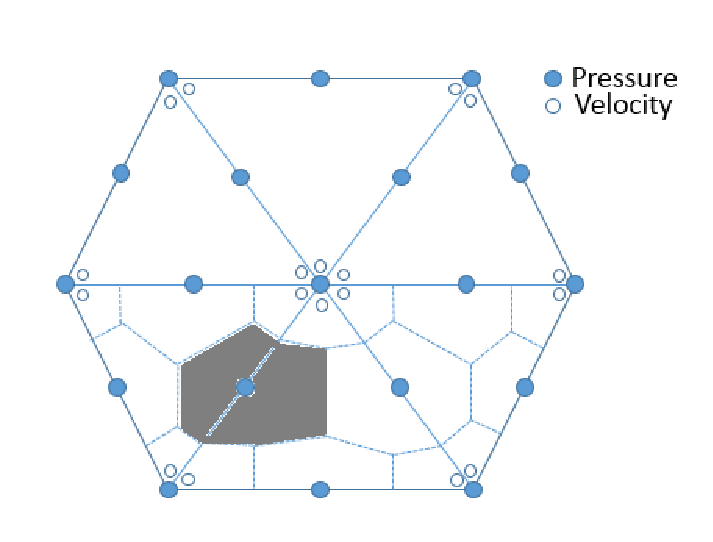
\includegraphics[width=.5\textwidth]{./Pics/P1DGP2.pdf}}
\caption{2D representation of \PN[1]{2} element pairs used in this work. Shaded areas denote control volumes across two contiguous elements. Blue and white circles represent pressure and velocity nodes, respectively.}
\label{fig:fem_cv}
\end{figure}

\clearpage

%%%%
%%%%  FIGURE
%%%%
\begin{figure}[h]
\centering
\vbox{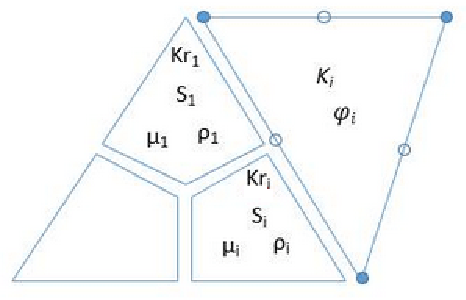
\includegraphics[width=.75\textwidth]{./Pics/element_n.pdf}}
\caption{This is a graphical representation of two different element types. Element A is the \PN[1]{2}, while element B is the \PN[1]{1}. Porosity $\phi_{i}$ and permeability $K_{i}$ are CV-wise quantities, whereas velocity and pressure are primarily represented in FE space. Scalar fields (such saturation, density, viscosity etc) are also represented in CV space.}
\label{fig:fem_elem}
\end{figure}
\clearpage

%%%%
%%%%  FIGURE 
%%%%
\begin{figure}[h]
\centering
\vbox{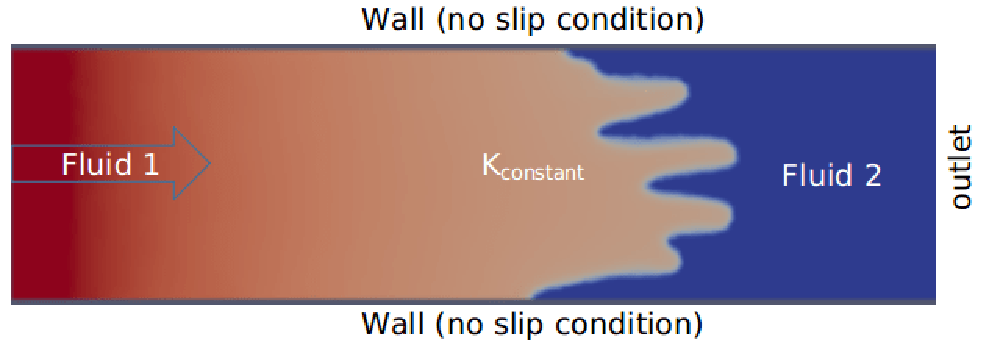
\includegraphics[width=0.75\textwidth]{./Pics/phase_vol_frac_uni_perm_1.pdf}}
\caption{Schematics of formation of flow instabilities during injection of a pure low viscosity fluid (red) into a domain saturated with a second fluid (dark blue). The ratio of viscosity between the two fluids is 5. In this case, the initially piston shape front collapses leading to the formation of several fingers.}
\label{fig:simple_case}
\end{figure}
\clearpage


%%%%
%%%%  FIGURE 
%%%%
\begin{figure}[ht] 
\vbox{
\hbox{\hspace{-0.3cm}
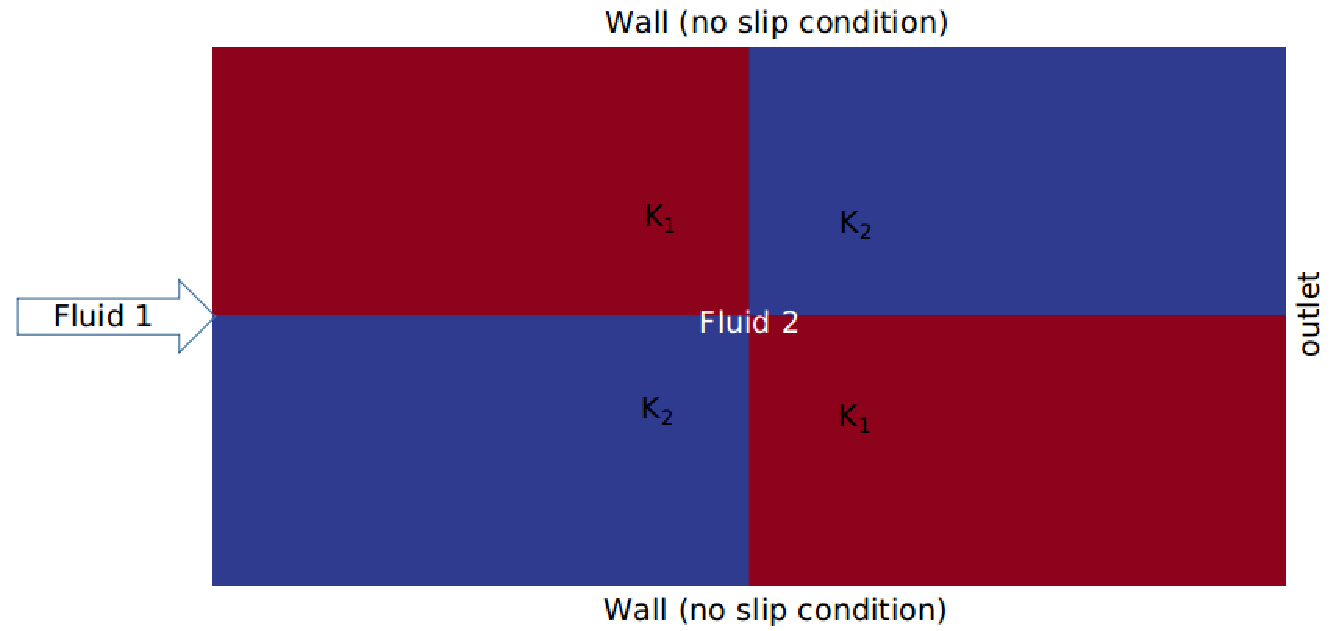
\includegraphics[width=.8\textwidth]{./Pics1/2b2_wi_fine/2b2_whole_in_fine_perm_1.pdf} 
}
\vspace{0.0cm}
\hbox{\hspace{3.5cm} (a) map of permeabilities ($\mathbf{K}$)
}
\vspace{0.25cm}
\hbox{\hspace{1.5cm}
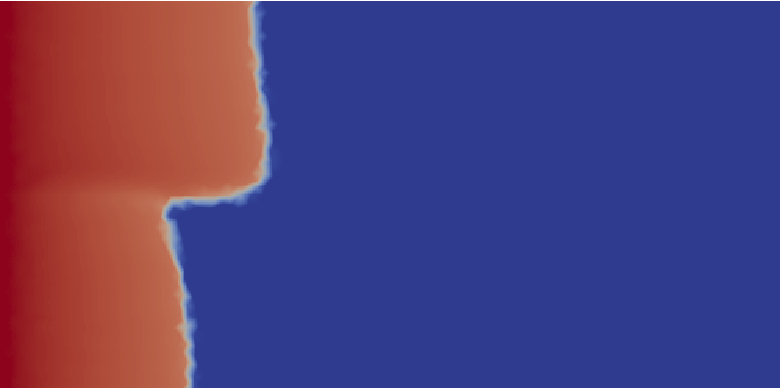
\includegraphics[width=.9\textwidth]{./Pics1/2b2_wi_fine/2b2_whole_in_fine_250_2.pdf}
}
\vspace{0.0cm}
\hbox{\hspace{4.5cm} (b) flow at t=250  
}
\vspace{0.25cm}
\hbox{\hspace{1.5cm}
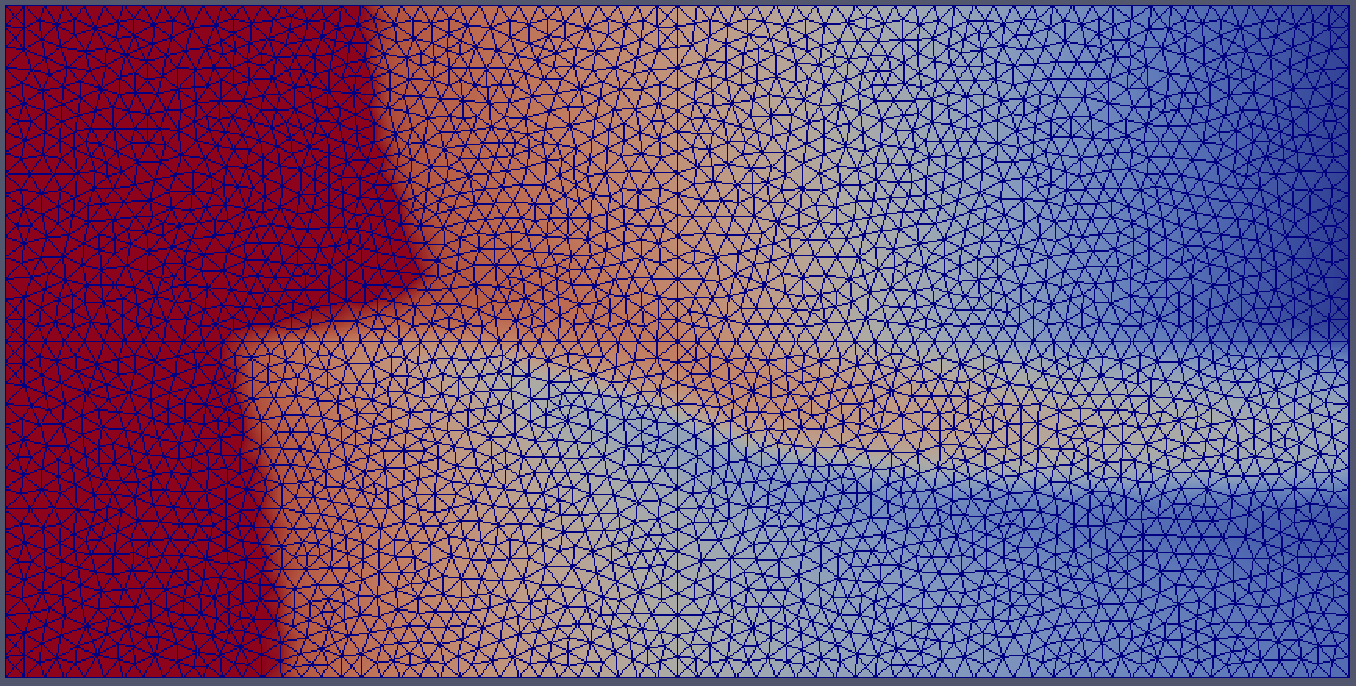
\includegraphics[width=.65\textwidth]{./Pics1/2b2_wi_fine/2b2_whole_in_fine_3000_1.pdf}
}
\vspace{0.0cm}
\hbox{\hspace{4.0cm} (c) flow at t=3000  
}
}     
\caption{Model validation of fluid displacement in heterogeneous porous media: (a) the domain is divided into four subdomains with prescribed synthetic permeability, $\mathbf{K}_{1}=1$ and $\mathbf{K}_{2}=2.5$; (b-c) snapshots of saturation (displacing fluid) field at $t=250$ and $t=3000$ sec. The domain is discretised with $5960$ \PN[1]{2} elements. }
\label{fem_cv_represent_a}
\end{figure}
\clearpage



%%%
%%% FIGURE
%%%
\begin{landscape}
  \begin{figure}[ht]
    \vbox{ 
      \hbox{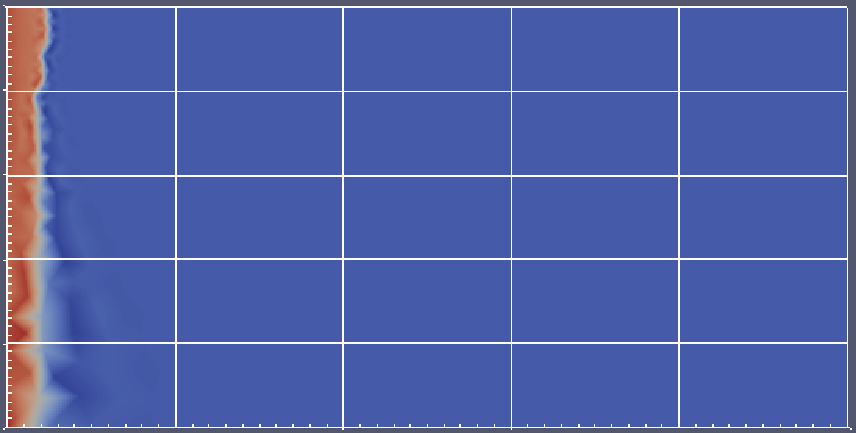
\includegraphics[width=.45\textwidth]{./Pics1/mr1_fixed/mr1_fixed_100_2.pdf}
            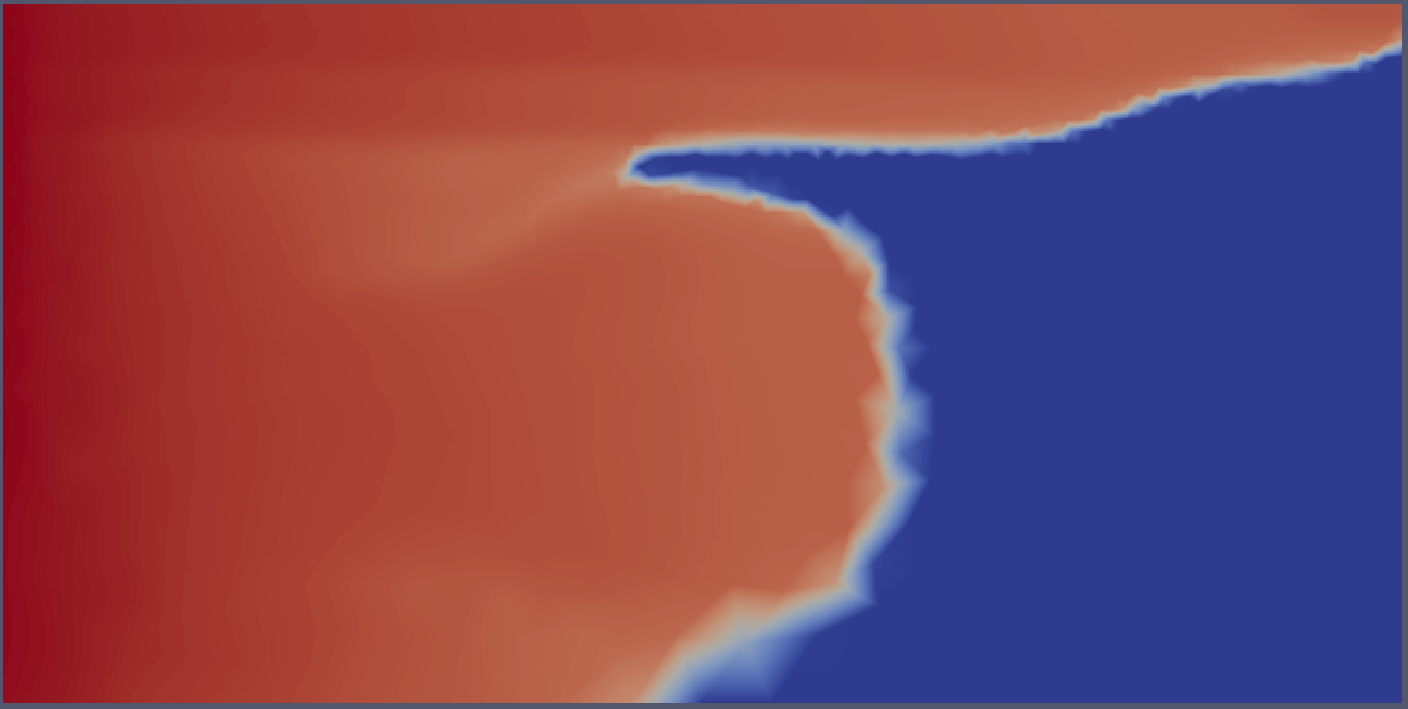
\includegraphics[width=.45\textwidth]{./Pics1/mr1_fixed/mr1_fixed_middle_1.pdf} 
            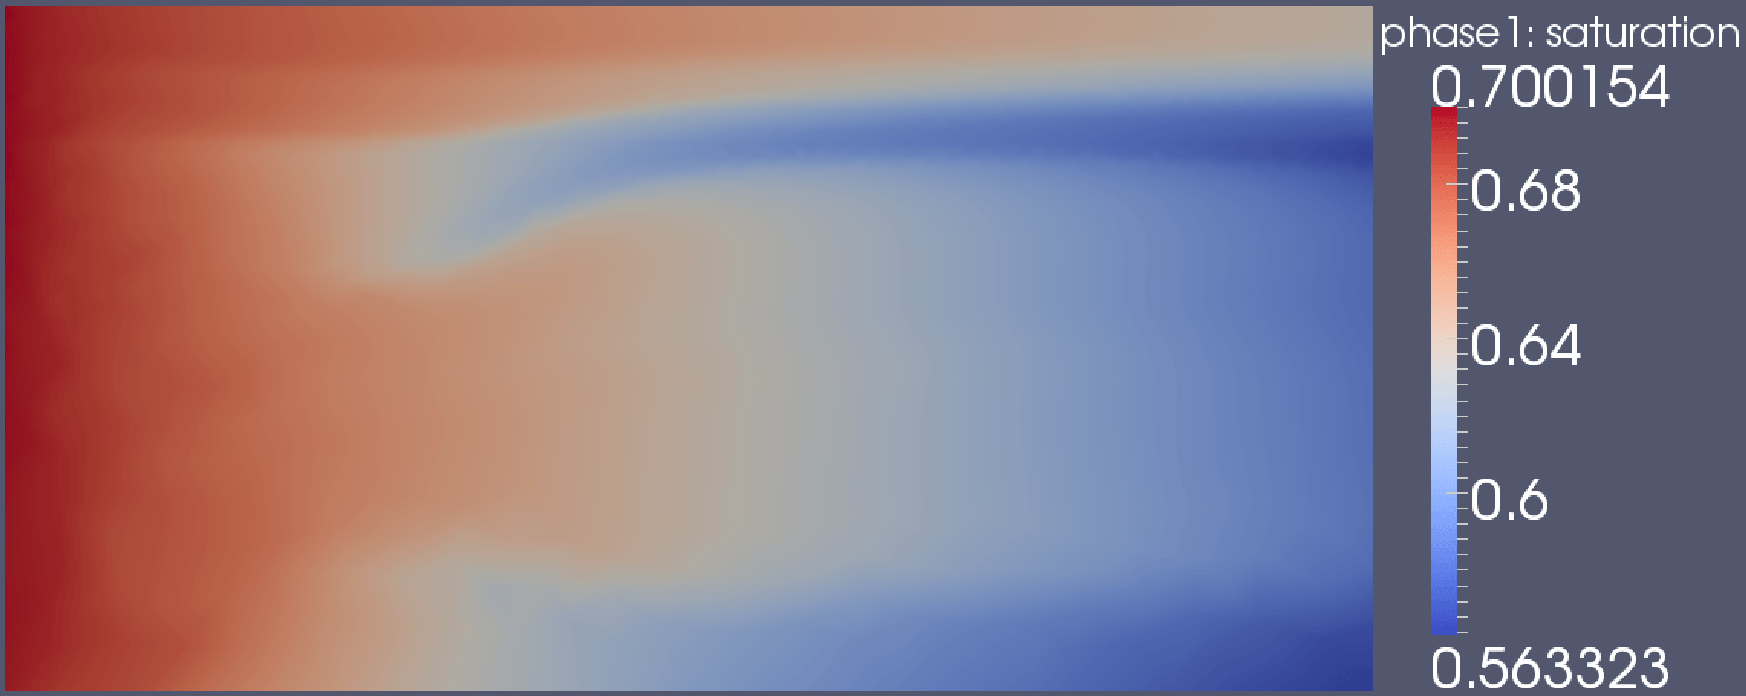
\includegraphics[width=.57\textwidth]{./Pics1/mr1_fixed/mr1_fixed_end_2.pdf} }
      \hbox{\hspace{8.0cm} (a) VR = 1}
      \vspace{1cm}
      \hbox{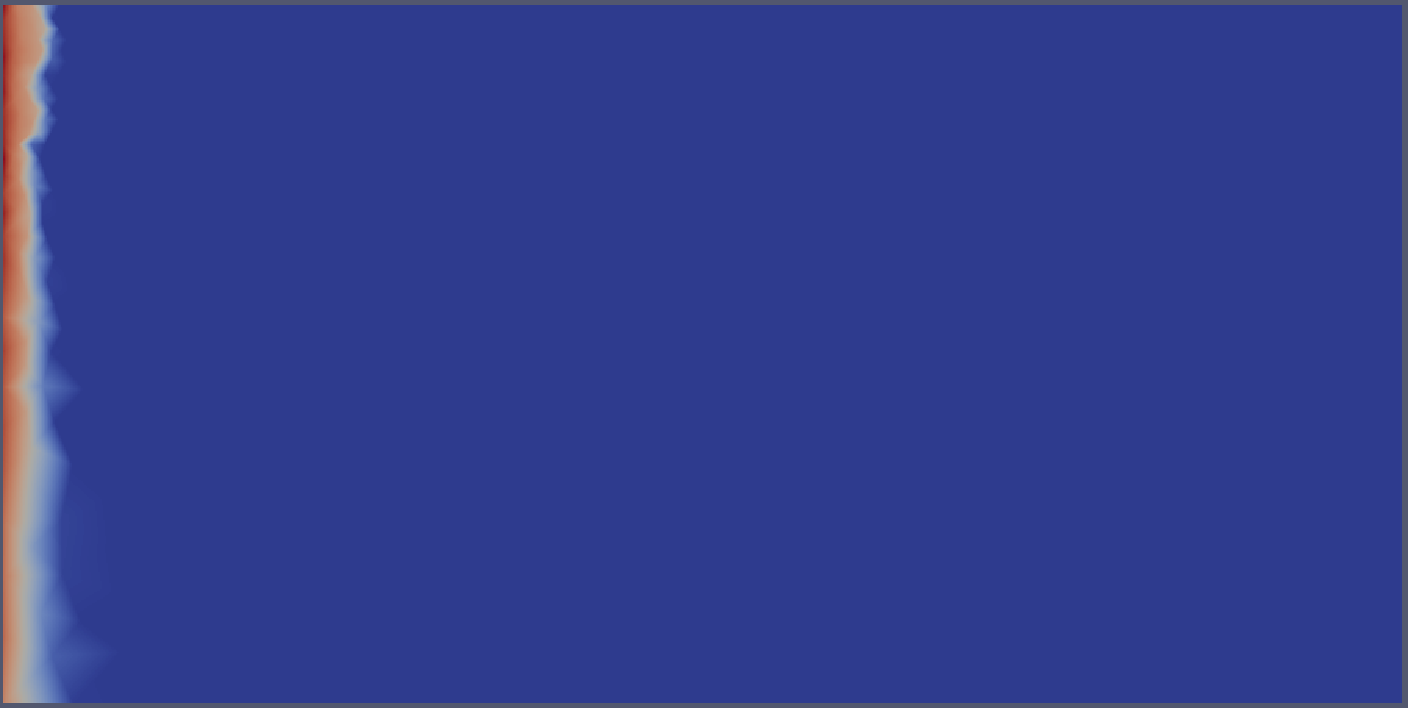
\includegraphics[width=.45\textwidth]{./Pics1/mr10_fixed/mr10_fixed_100_1.pdf}
            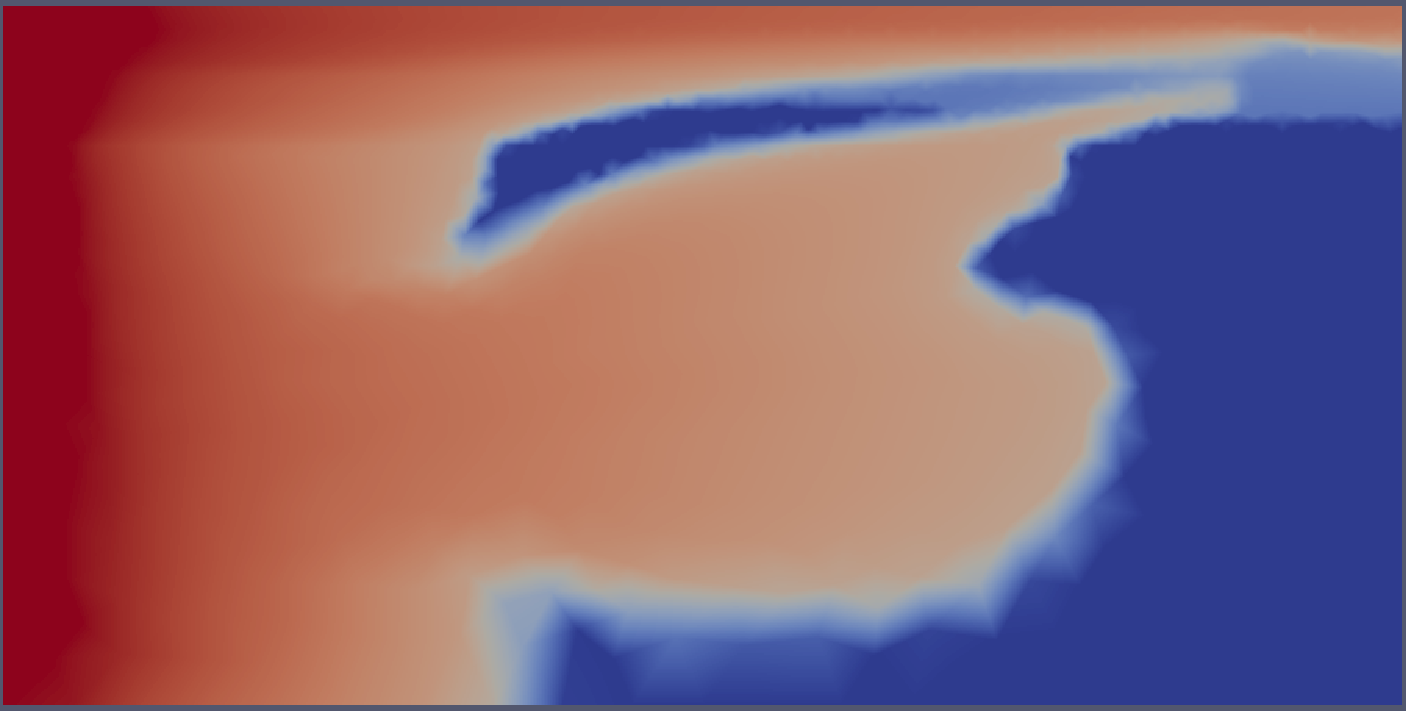
\includegraphics[width=.45\textwidth]{./Pics1/mr10_fixed/mr10_fixed_middle_1.pdf}
            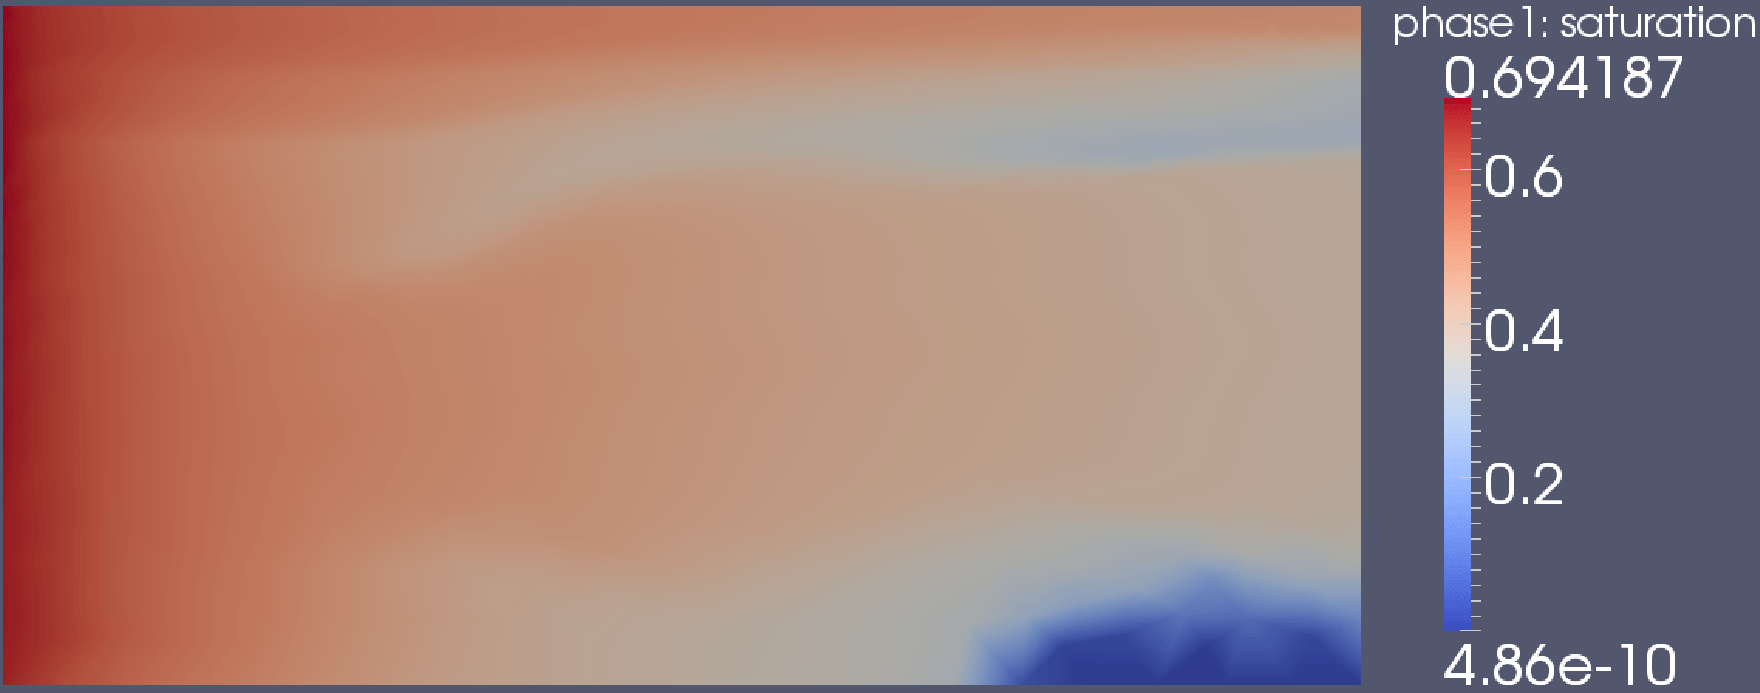
\includegraphics[width=.57\textwidth]{./Pics1/mr10_fixed/mr10_fixed_end_2.pdf} }
      \hbox{\hspace{8.0cm} (b) VR = 10  }}
\caption{Initial model validation: snapshots of numerical simulations performed with VR=1 and VR=10. The domain contains $4700$ elements.}
\label{fem_cv_represent_vr1_vr10}
\end{figure}
\end{landscape}
\clearpage
%%%
%%%
%%%



%%%%
%%%%  FIGURE
%%%%
\begin{landscape}
\begin{figure}[ht] 
\vbox{\vspace{-1cm}
\hbox{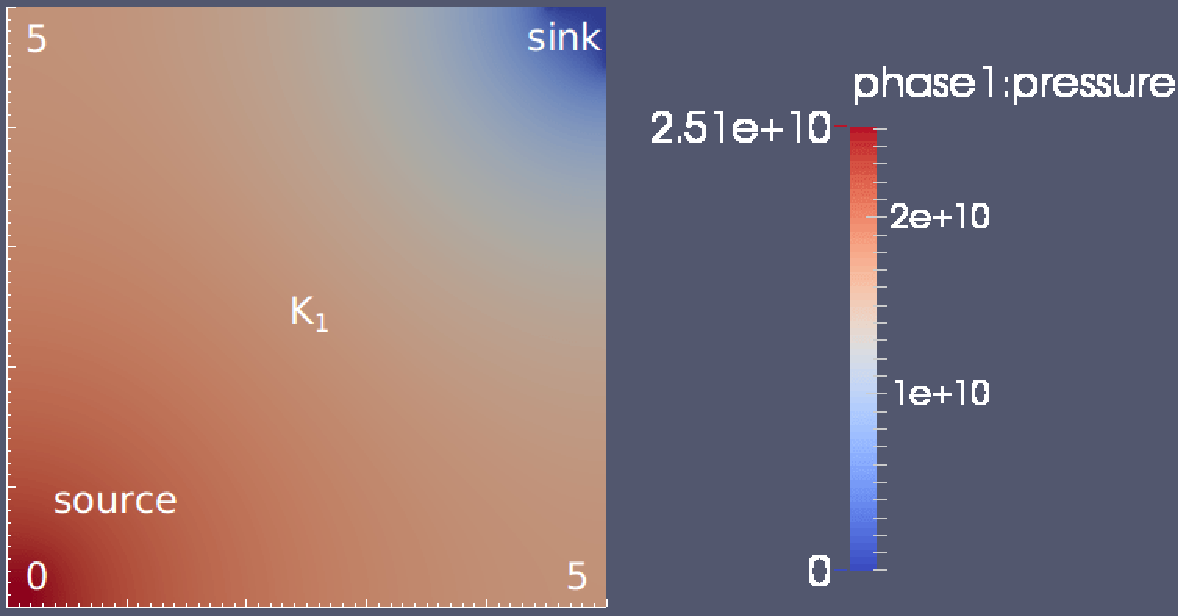
\includegraphics[width=.7\textwidth]{./Pics1/Saffman_homogeneous_MR3/saffman_homo_fixed_2.pdf}
      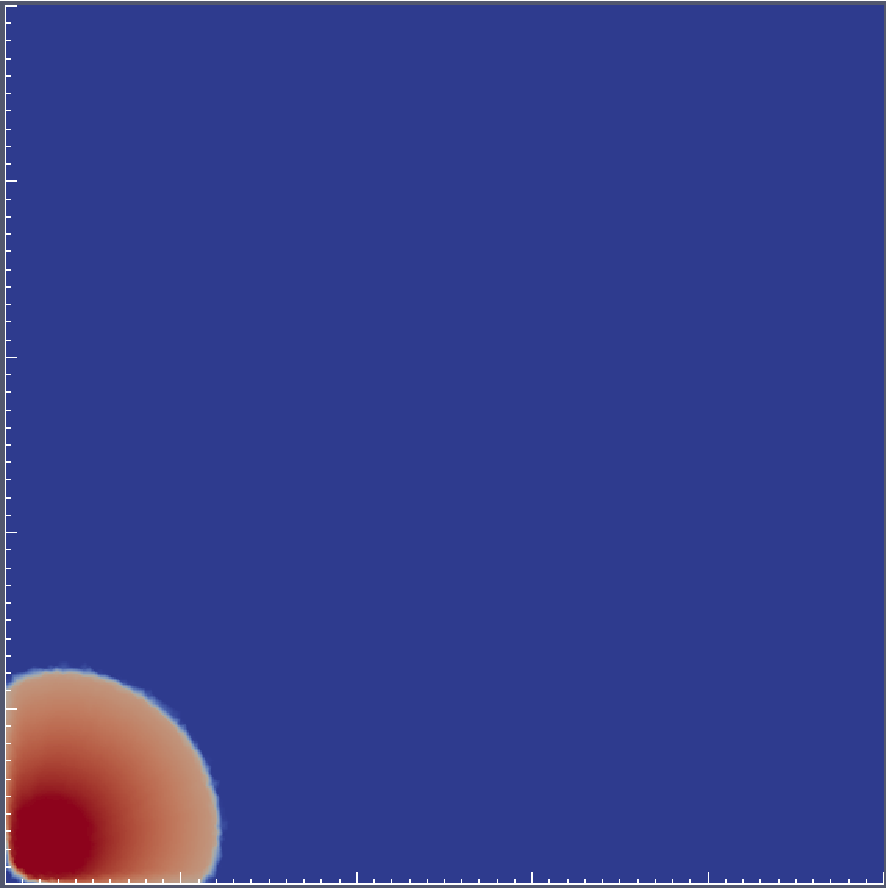
\includegraphics[width=.37\textwidth]{./Pics1/Saffman_homogeneous_MR3/saffman_homo_fixed_250.pdf}
      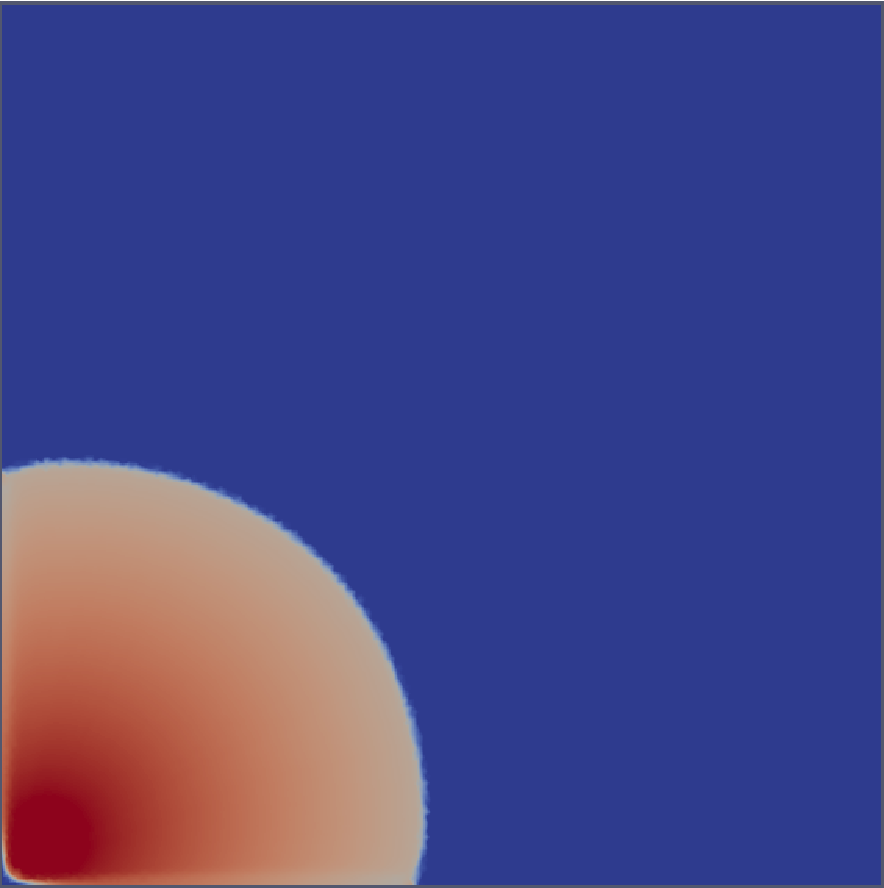
\includegraphics[width=.37\textwidth]{./Pics1/Saffman_homogeneous_MR3/saffman_homo_fixed_1000.pdf}}
\vspace{0.cm}
\hbox{\hspace{2.5cm} (a) pressure at t=0s \hspace{5.cm} (b) t=0.87s \hspace{2.75cm} (c) t=3.54s}
\vspace{0.5cm}
\hbox{
      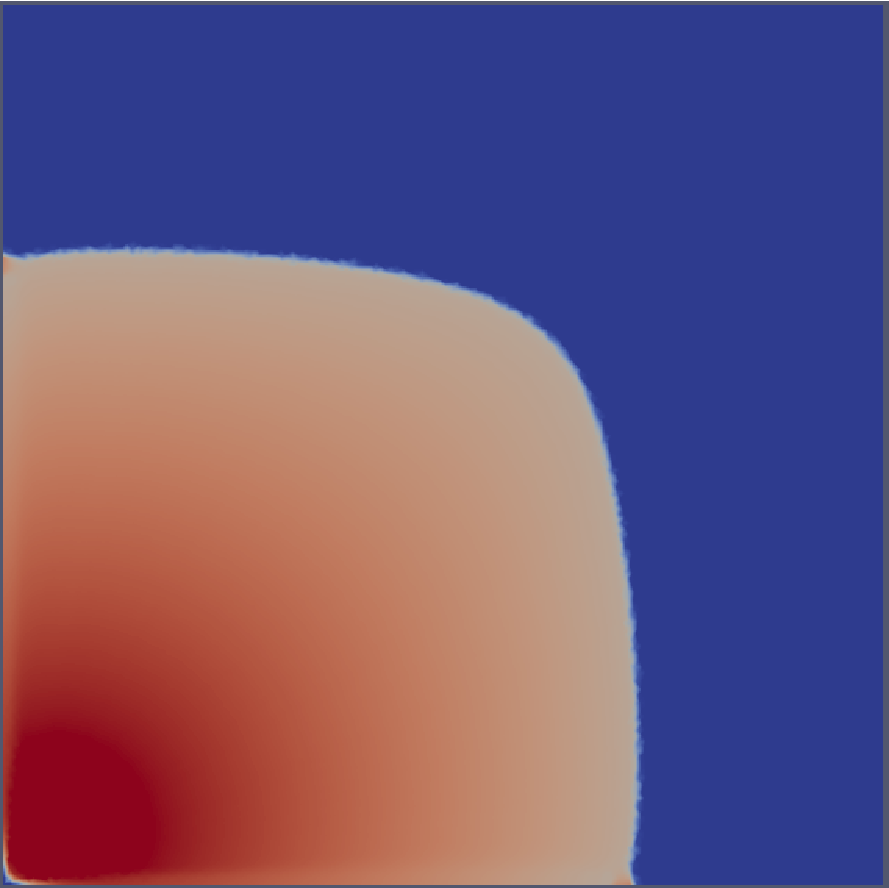
\includegraphics[width=.375\textwidth]{./Pics1/Saffman_homogeneous_MR3/saffman_homo_fixed_2500.pdf}
      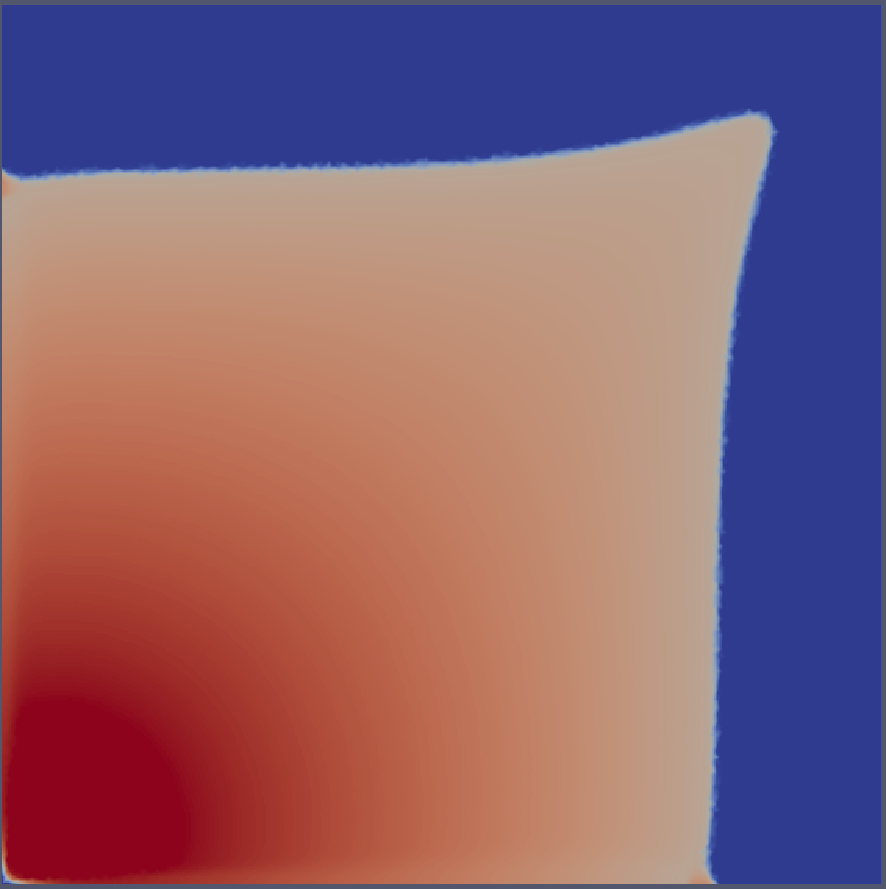
\includegraphics[width=.375\textwidth]{./Pics1/Saffman_homogeneous_MR3/saffman_homo_fixed_3500.pdf} 
      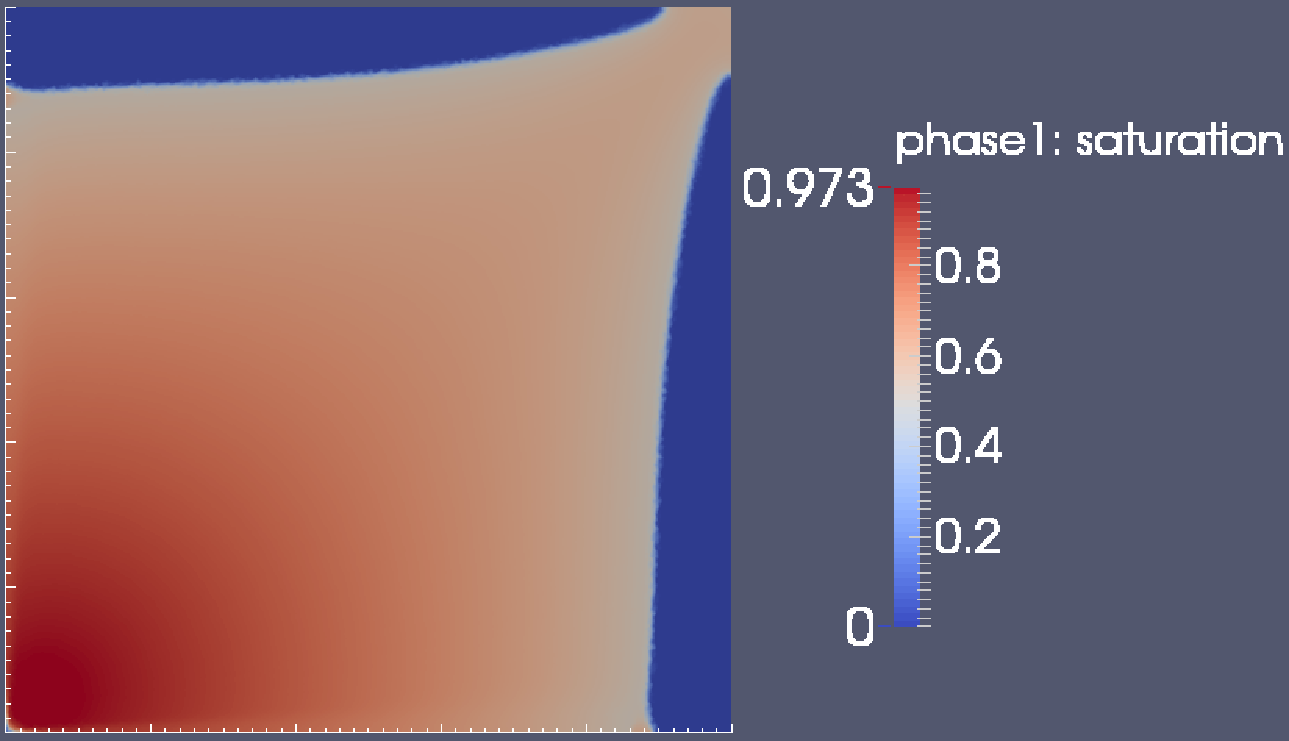
\includegraphics[width=.65\textwidth]{./Pics1/Saffman_homogeneous_MR3/saffman_homo_fixed_end.pdf}}
\vspace{0.cm}
\hbox{ \hspace{1.cm} (d) t=8.86s \hspace{3.0cm} (e) t=12.41s   \hspace{4.0cm} (f) t=17.95s}
\vspace{0.cm}
}   
\caption{Simulated flow in a Hele-Shaw cell ({\it VR}=3): (a) initial pressure profile $\left(\text{in g.cm}^{-1}\text{.s}^{-2}\right)$ with source and sink regions are explicitly shown along with dimensions (in cm); (b-f) snapshots of wetting phase saturation showing flow profile as the simulation evolves. The domain contains $47500$ \PN[1]{2} triangular elements.}
\label{fig:homoheleshaw_VN3}
\end{figure}
\end{landscape}
\clearpage



%%%%
%%%%  FIGURE
%%%%
\begin{landscape}
\begin{figure}[ht] 
\vbox{\vspace{-1cm}
\hbox{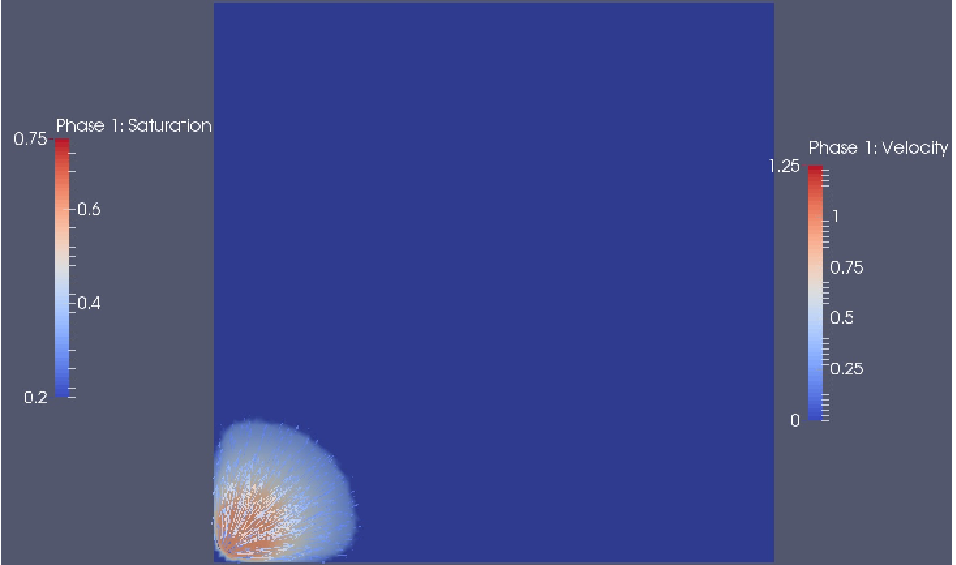
\includegraphics[width=.9\textwidth, height=0.5\textwidth]{./Pics1/Saffman_homogeneous_VR10/ST_Homog_VR10_D201c}
\hspace{0.5cm}      
      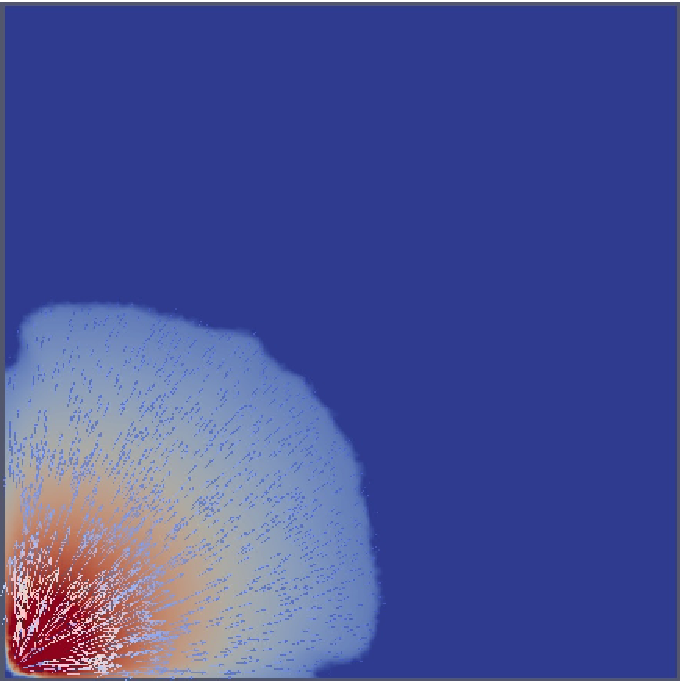
\includegraphics[width=.5\textwidth]{./Pics1/Saffman_homogeneous_VR10/ST_Homog_VR10_D1001c}}
\vspace{0.cm}
\hbox{\hspace{5.cm} (a) t=0.66s \hspace{8.cm} (b) t=3.43s }
\vspace{0.5cm}
\hbox{
      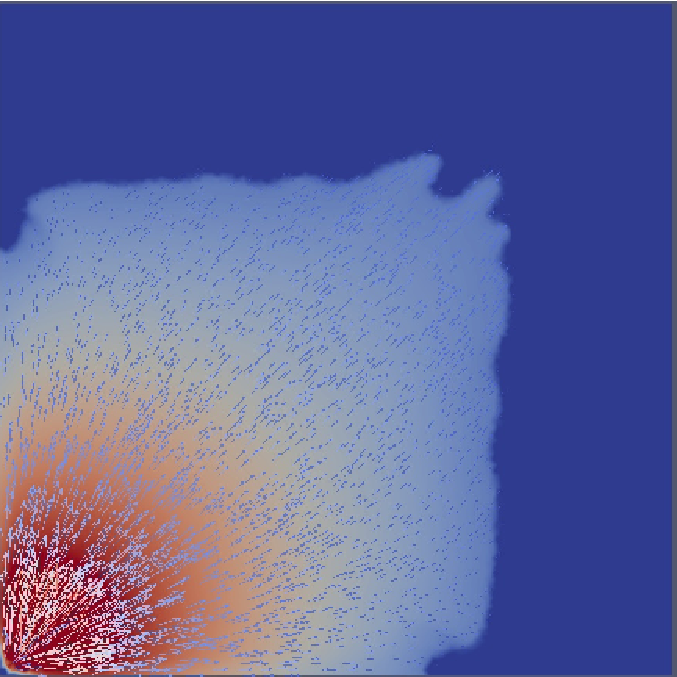
\includegraphics[width=.5\textwidth]{./Pics1/Saffman_homogeneous_VR10/ST_Homog_VR10_D2001c}
      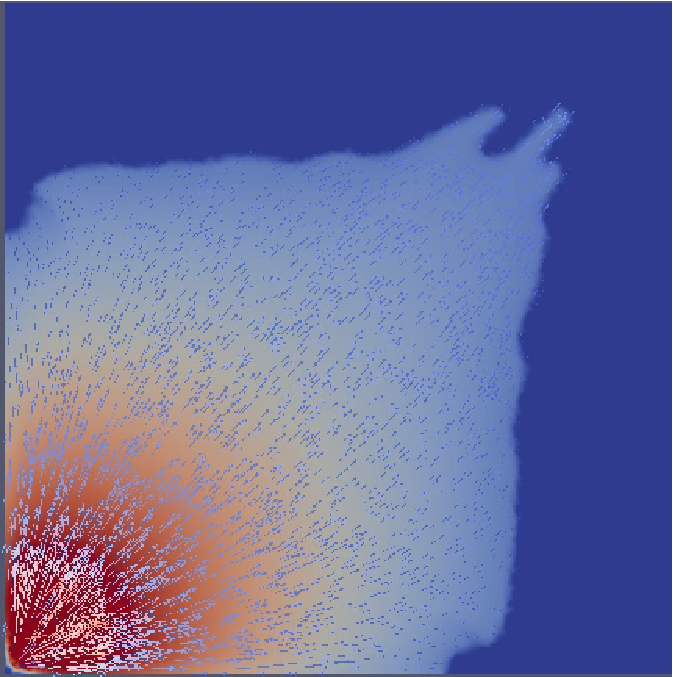
\includegraphics[width=.5\textwidth]{./Pics1/Saffman_homogeneous_VR10/ST_Homog_VR10_D2201c}
      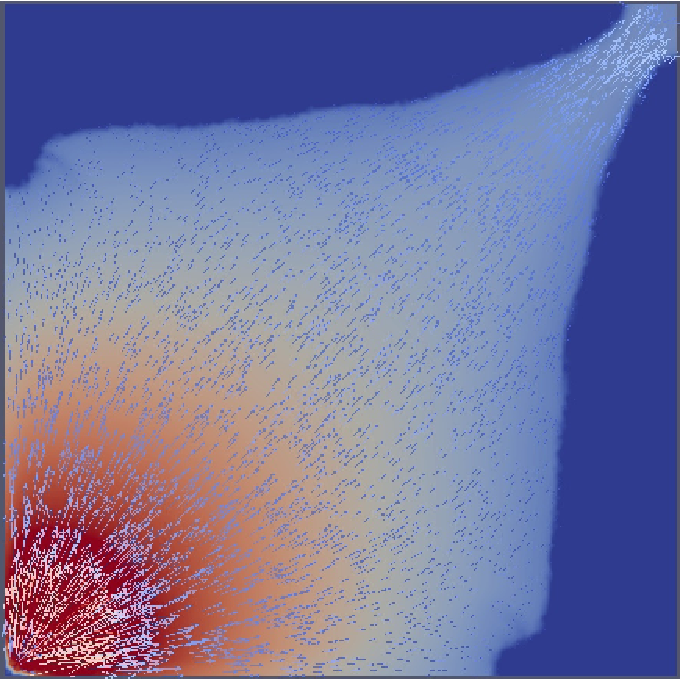
\includegraphics[width=.5\textwidth]{./Pics1/Saffman_homogeneous_VR10/ST_Homog_VR10_D3001c}}
\vspace{0.cm}
\hbox{ \hspace{2.cm} (c) t=6.92s \hspace{4.5cm} (d) t=7.61s \hspace{4.5cm} (e)t=10.00s}
\vspace{0.cm}
}   
\caption{Simulated flow in a Hele-Shaw cell ({\it VR}=10): snapshots of overlapped wetting phase saturation and velocity vectors showing flow profile as the simulation evolves. The domain contains $26313$ \PN[1]{2} triangular elements.}
\label{fig:homoheleshaw_VN10}
\end{figure}
\end{landscape}
\clearpage





\begin{comment}

%%%%
%%%%  FIGURE
%%%%
\begin{landscape}
\begin{figure}[ht] 
\vbox{\vspace{-1cm}
\hbox{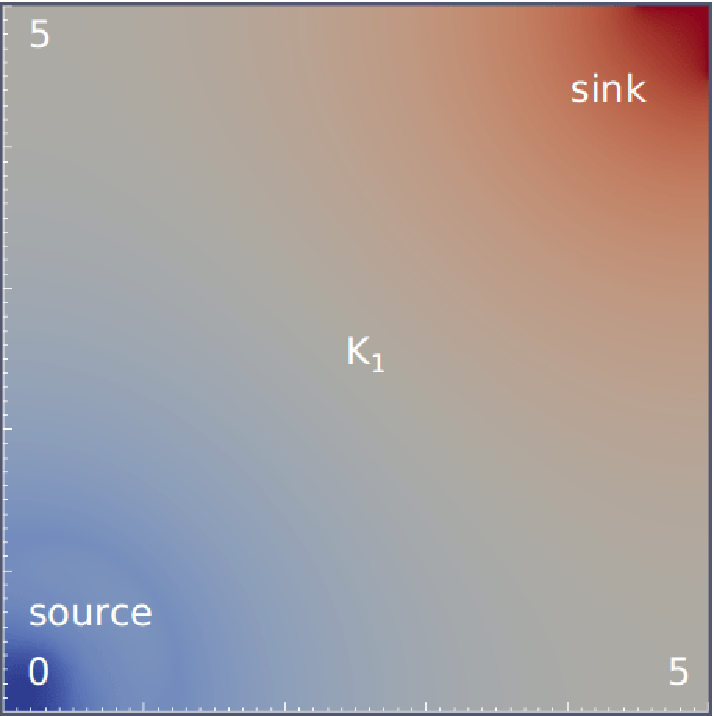
\includegraphics[width=.5\textwidth]{./Pics1/Saffman_homogeneous/saffman_homo_fixed_1.pdf}
      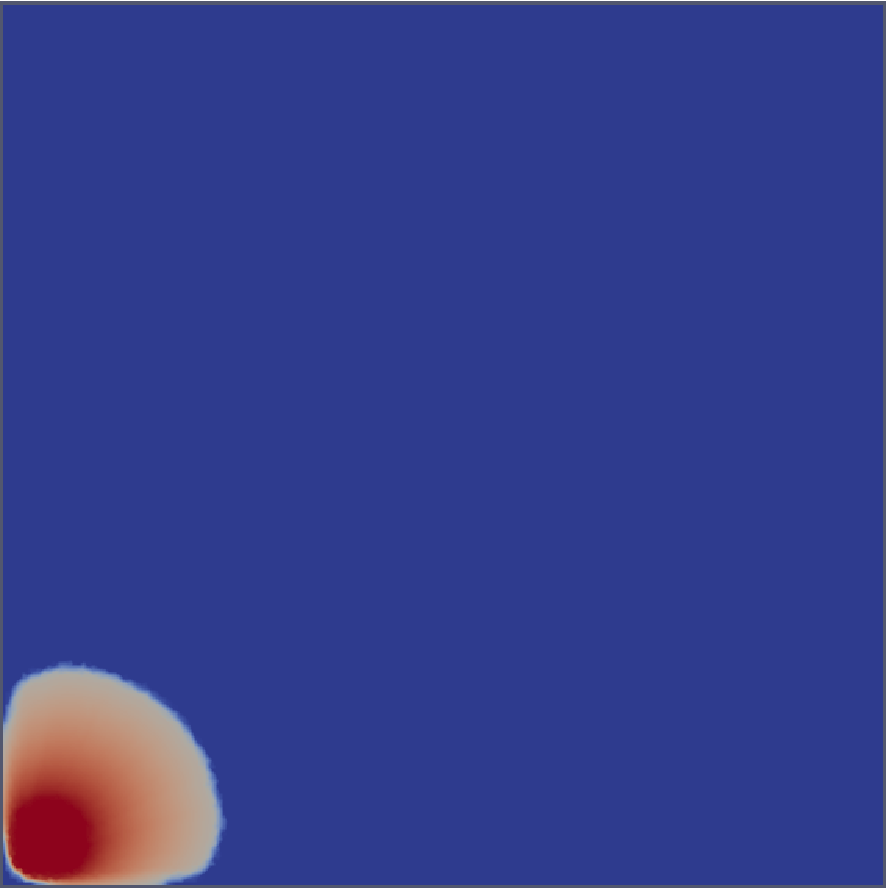
\includegraphics[width=.5\textwidth]{./Pics1/Saffman_homogeneous/saffman_homo_fixed_250_1.pdf}
      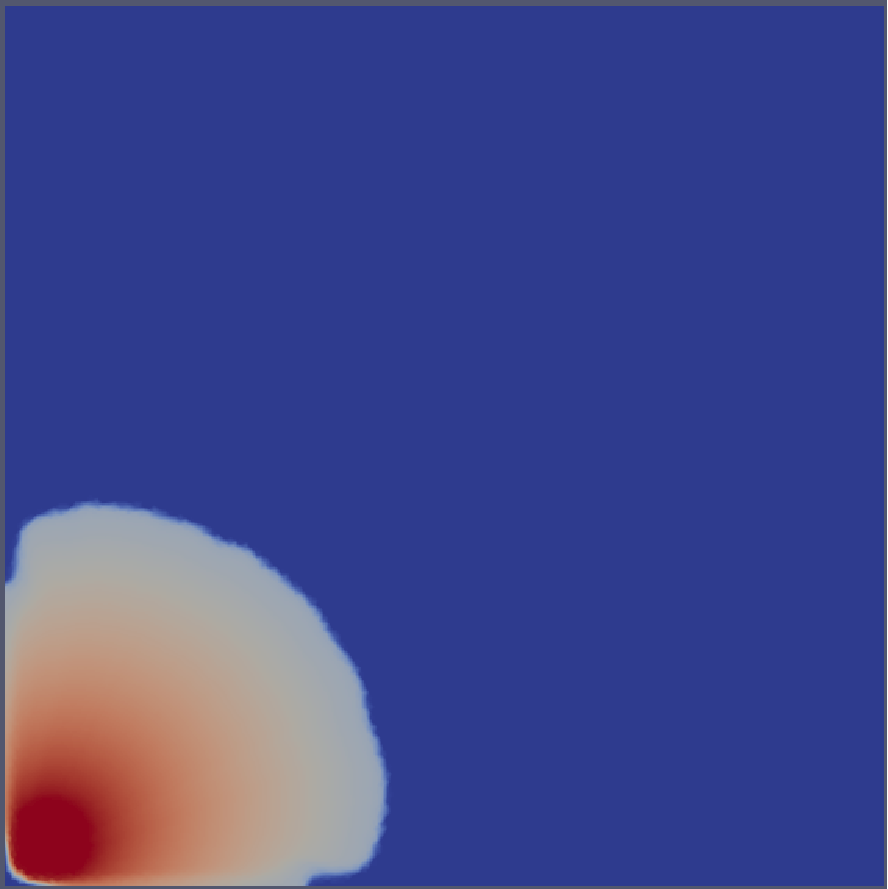
\includegraphics[width=.5\textwidth]{./Pics1/Saffman_homogeneous/saffman_homo_fixed_1000.pdf}}
\vspace{0.cm}
\hbox{\hspace{1.0cm} (a) pressure at t=0 \hspace{3.cm} (b) t=250\red{(???)} \hspace{3.0cm} (c) t=1000\red{(???)}}
\vspace{0.5cm}
\hbox{
      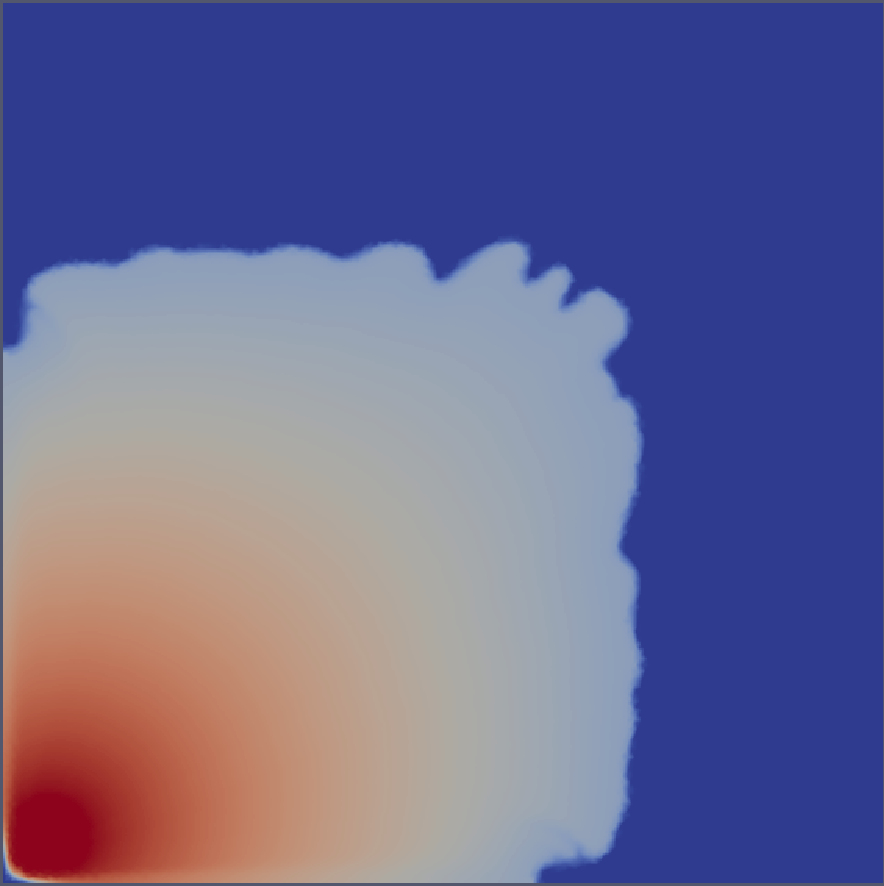
\includegraphics[width=.5\textwidth]{./Pics1/Saffman_homogeneous/saffman_homo_fixed_6000.pdf}
      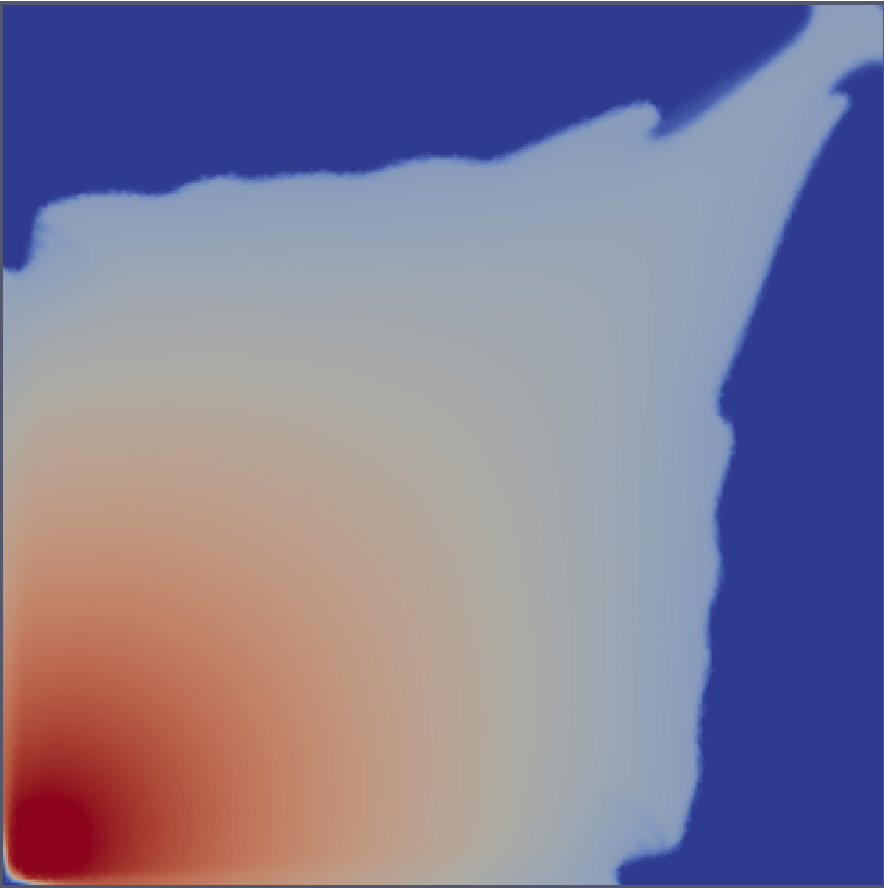
\includegraphics[width=.5\textwidth]{./Pics1/Saffman_homogeneous/saffman_homo_fixed_end_1.pdf}}
\vspace{0.cm}
\hbox{ \hspace{2.cm} (d) t=6000\red{(???)} \hspace{3.cm} (e) t=XXX\red{(???)}}
\vspace{0.cm}
}   
\caption{Simulated flow in a Hele-Shaw cell ({\it VR}=10): (a) pressure profile $\left(\text{in g.cm}^{-1}\text{.s}^{-2}\right)$ with source and sink regions explicitly shown along with dimensions (in cm); (b-e) snapshots of wetting phase saturation showing flow profile as the simulation evolves. The domain contains $47000$ \PN[1]{2} triangular elements. The pressure and saturation range of values are the same like the  case in fig.\ref{fig:homoheleshaw_VN3}.}
\label{fig:homoheleshaw_VN10}
\end{figure}
\end{landscape}
\clearpage
\end{comment}


%%%
%%% FIGURE XXXXXX
%%%
\begin{landscape}
  \begin{figure}[ht]
  \vbox{\vspace{-1cm}
      \hbox{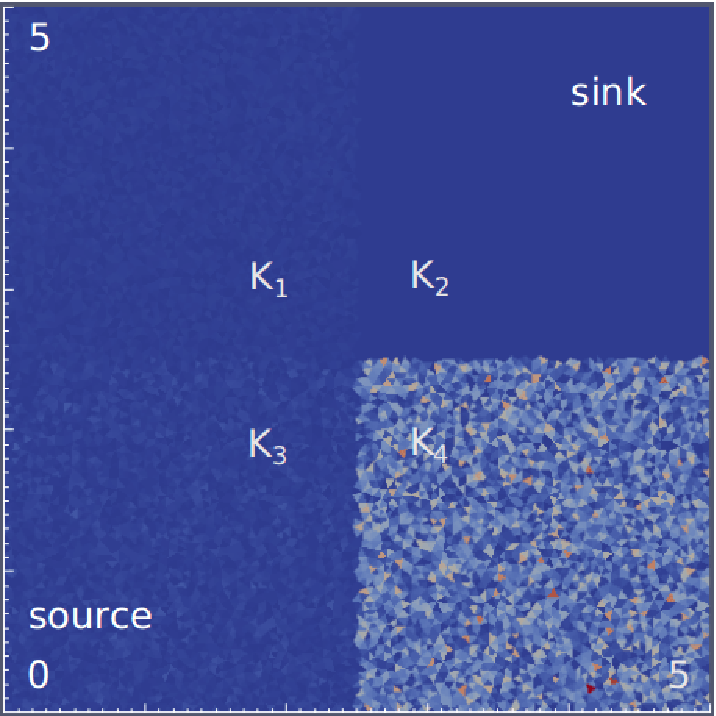
\includegraphics[width=.5\textwidth]{./Pics1/Saffman_heterogeneous/saffman_heter_fixed_1.pdf}
            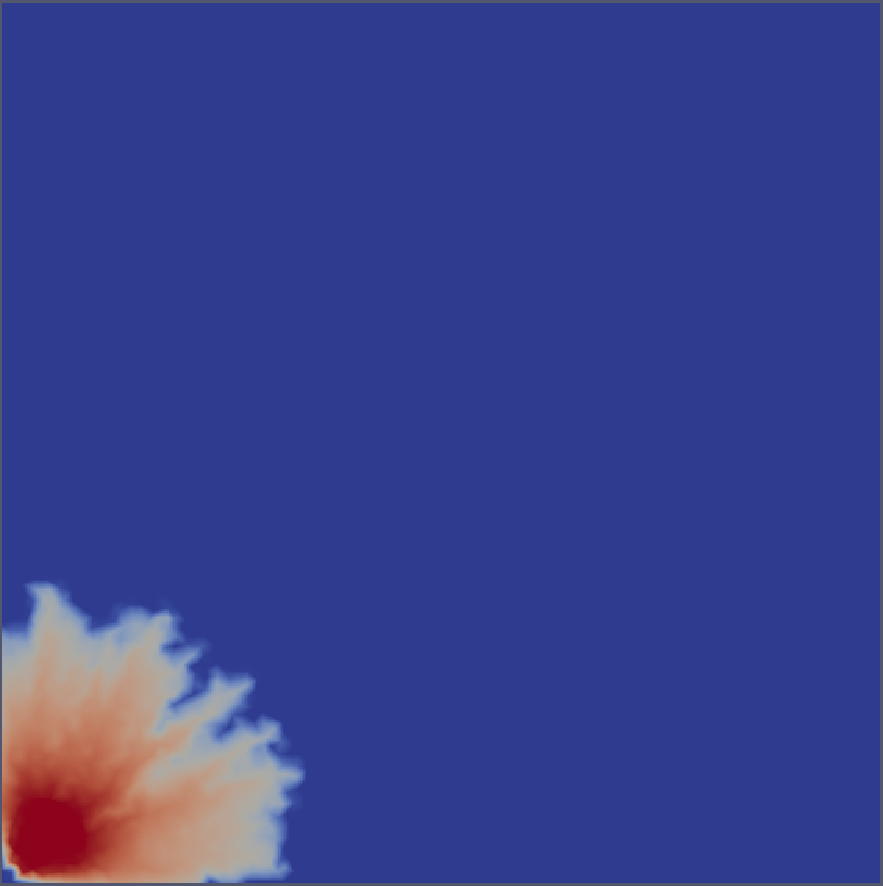
\includegraphics[width=.5\textwidth]{./Pics1/Saffman_heterogeneous/saffman_heter_fixed_500.pdf} 
            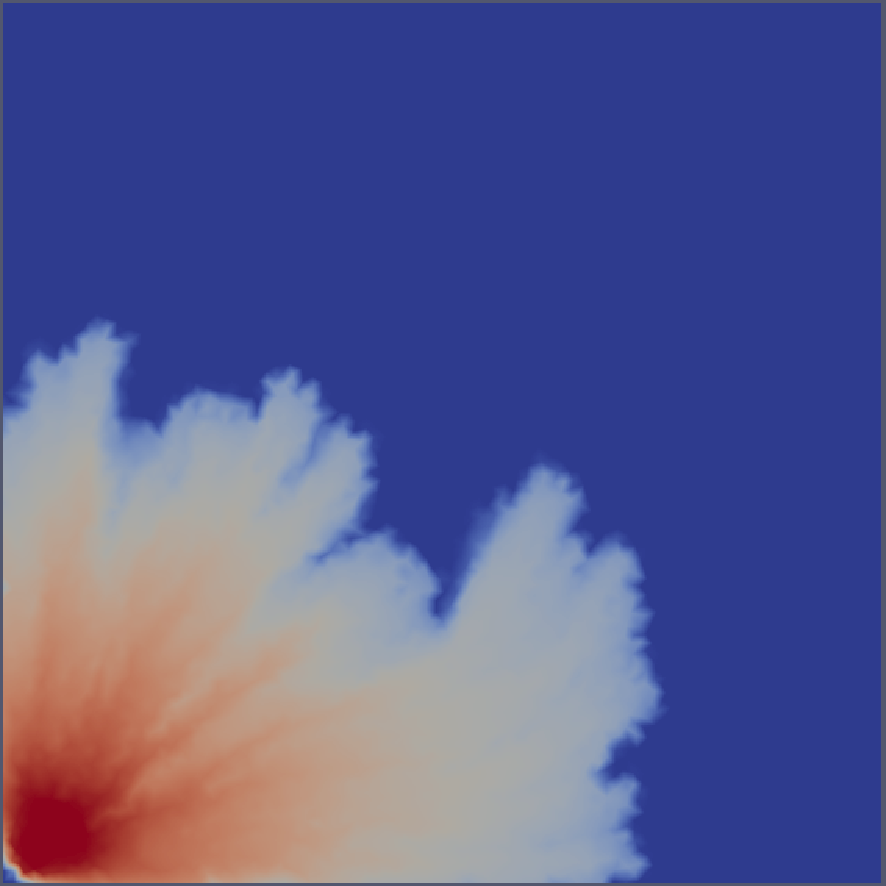
\includegraphics[width=.5\textwidth]{./Pics1/Saffman_heterogeneous/saffman_heter_fixed_2000.pdf} }
      \hbox{\hspace{1.0cm} (a) map of permeabilities \hspace{3.cm} (b) t=0.75s \hspace{4.0cm} (c) t=8s}
      \vspace{0.5cm}
      \hbox{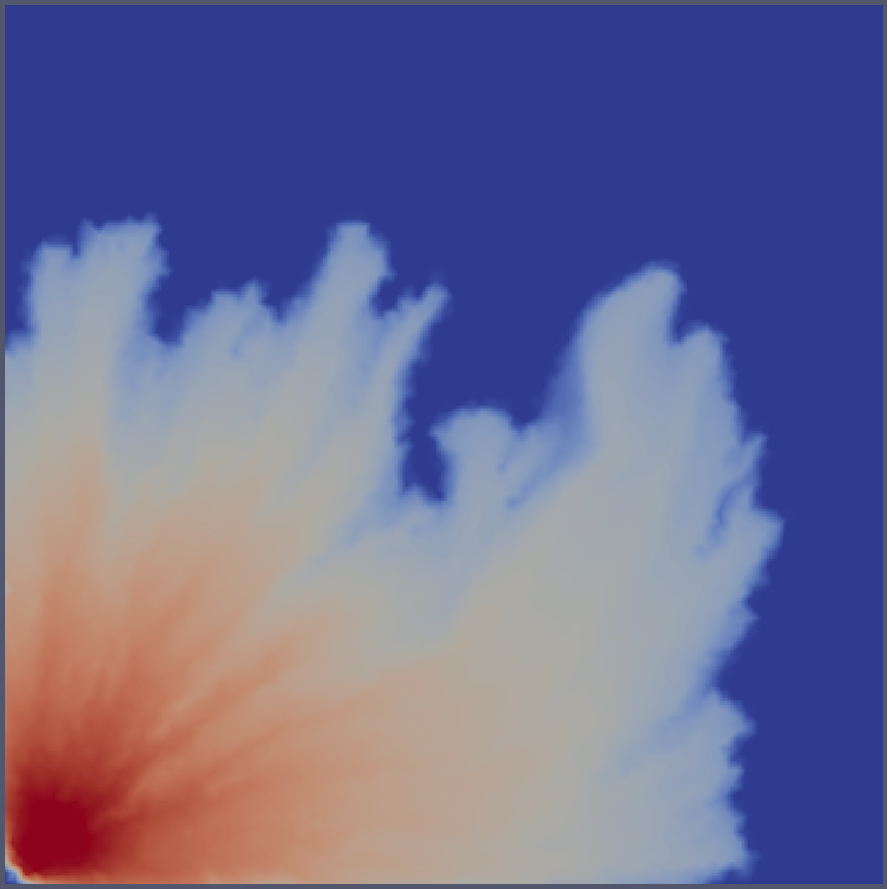
\includegraphics[width=.5\textwidth]{./Pics1/Saffman_heterogeneous/saffman_heter_fixed_3000.pdf}
            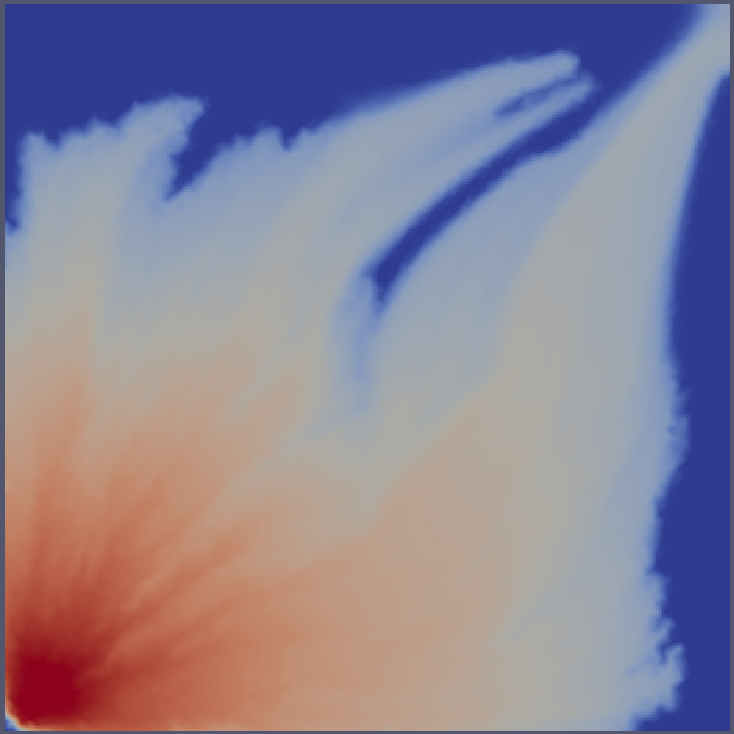
\includegraphics[width=.5\textwidth]{./Pics1/Saffman_heterogeneous/saffman_heter_fixed_6000.pdf}
            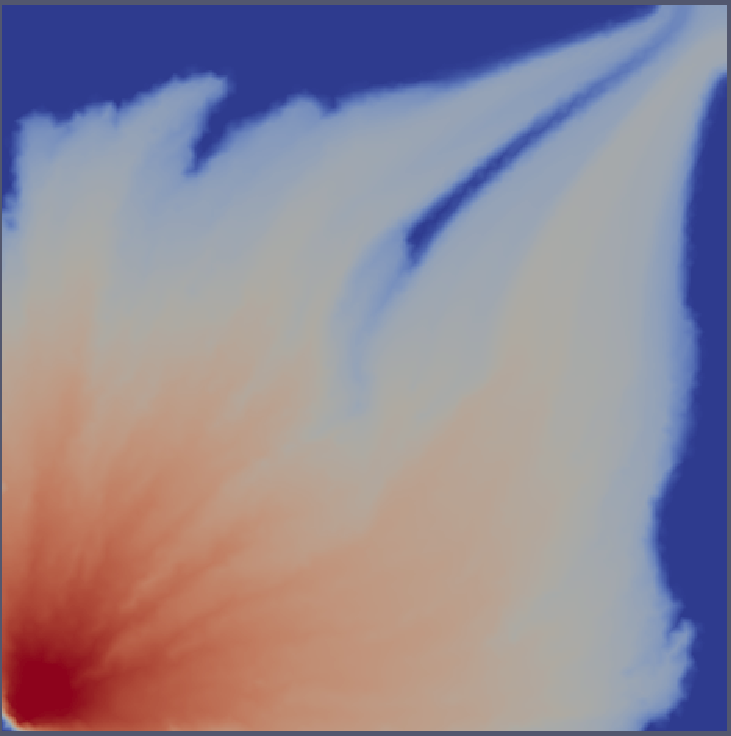
\includegraphics[width=.5\textwidth]{./Pics1/Saffman_heterogeneous/saffman_heter_fixed_24000.pdf} }
      \hbox{\hspace{2.5cm} (d) t=18s \hspace{5.cm} (e) t= \hspace{3.0cm} (f) t=24000 }}
\caption{Simulated flow in a modified Hele-Shaw cell with (a) prescribed distribution of permeability field $\left(\text{10}^{-10}\le\mathbf{K}_{1}\le\text{5}\times\text{10}^{-10}\right.$. The domain contains \red{XXXX} elements.}
\label{fig:HeleShawHeter_VR10}
\end{figure}
\end{landscape}
\clearpage



%%%%
%%%%  FIGURE
%%%%
\begin{landscape}
\begin{figure}[ht] 
\vbox{
\hbox{\hspace{4.0cm}
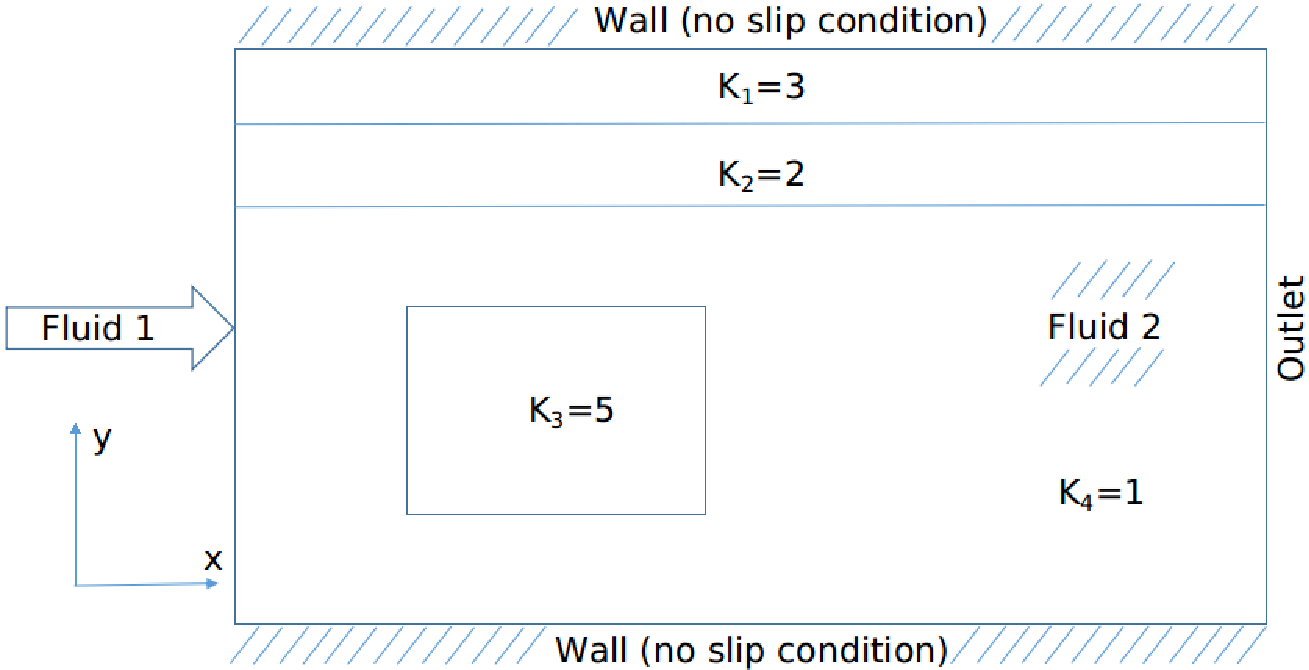
\includegraphics[width=.8\textwidth]{./Pics/map_of_boundaries.pdf} 
}
\vspace{0.0cm}
\hbox{\hspace{6.5cm} (a) map of permeabilties K   
}
\vspace{0.25cm}
\hbox{\hspace{4.0cm}
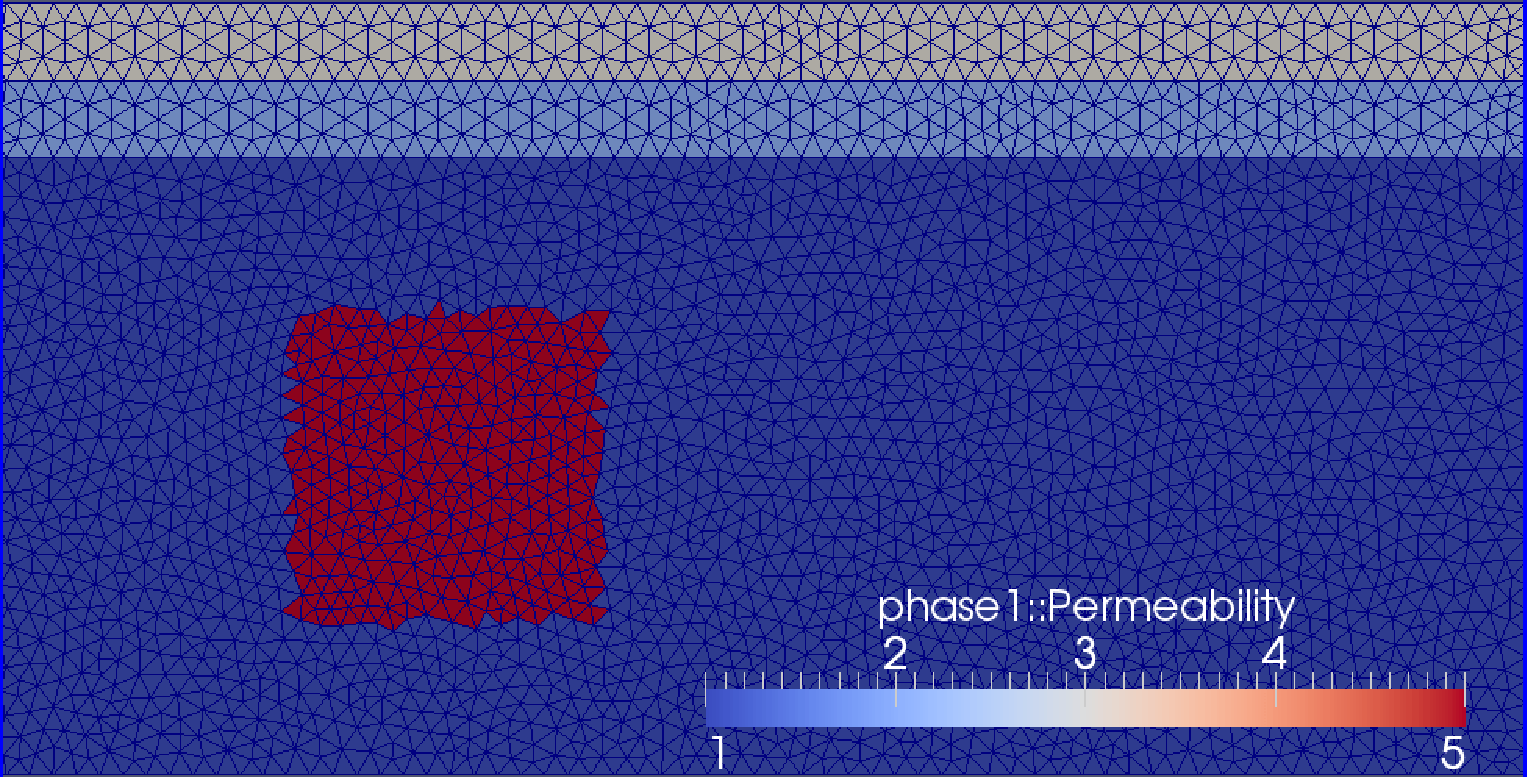
\includegraphics[width=.8\textwidth]{./Pics/4r_po_adapt_fine_125_mesh.pdf}
}
\vspace{0.0cm}
\hbox{\hspace{9cm} (b)      
}
}     
\caption{(a) describes the initial and boundary conditions as these are applied in this set of simulations. Below (b) the unstructured and fixed mesh can been seen and there is a colored representation of permeabilities.}
\label{fig:testcase_heter_domain}
\end{figure}
\end{landscape}
\clearpage


%%%%
%%%%  FIGURE
%%%%
\begin{landscape}
\begin{figure}[ht] 
\vbox{
\hbox{\hspace{3.5cm}
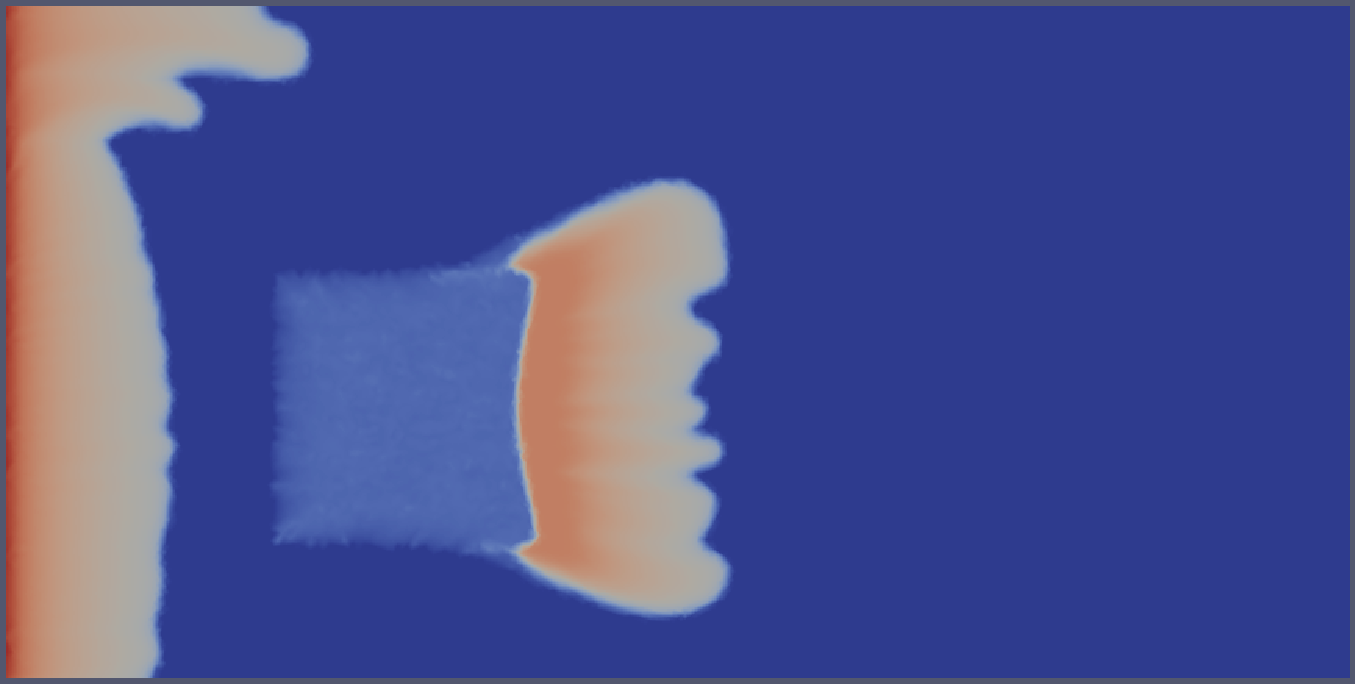
\includegraphics[width=.8\textwidth]{./Pics1/mr10_5regions_fixed/5regions_fixed_250.pdf} 
}
\vspace{0.0cm}
\hbox{\hspace{6.5cm} (a) flow at t=250 (fixed mesh)  
}
\vspace{0.25cm}
\hbox{\hspace{3.5cm}
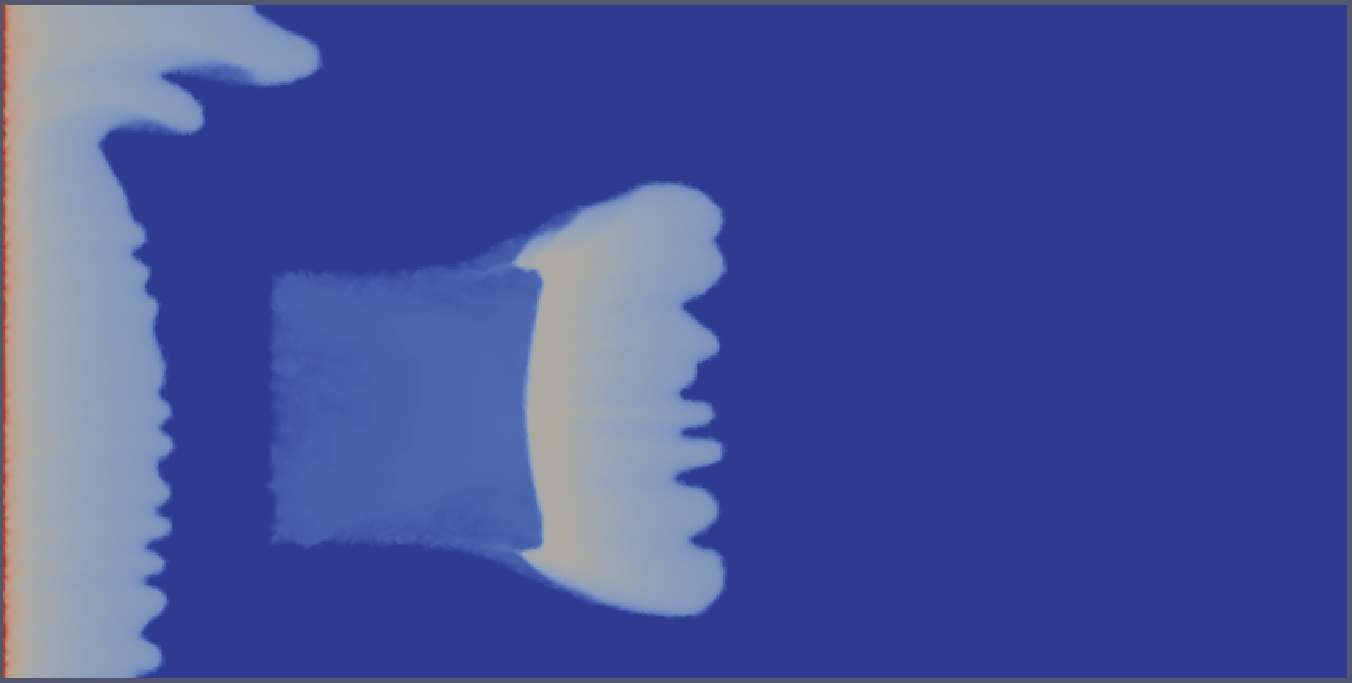
\includegraphics[width=.8\textwidth]{./Pics1/mr10_5regions_adapt/5regions_adapt_250.pdf}
}
\vspace{0.0cm}
\hbox{\hspace{6.5cm} (b) flow at t=250 (adaptive mesh)    
}
}     
\caption{Start to compare $2$ test-cases under MR=$10$ and under fixed (top) and adaptive(bottom) mesh for $time=0.125$ sec ($t=250$, timestemp). There is a significant difference on the main front (left hand side of the domain) and the number of finger that appear.}
\label{fig:2testcase_a}
\end{figure}
\end{landscape}
\clearpage


%%%%
%%%%  FIGURE
%%%%
\begin{landscape}
\begin{figure}[ht] 
\vbox{
\hbox{\hspace{3.5cm}
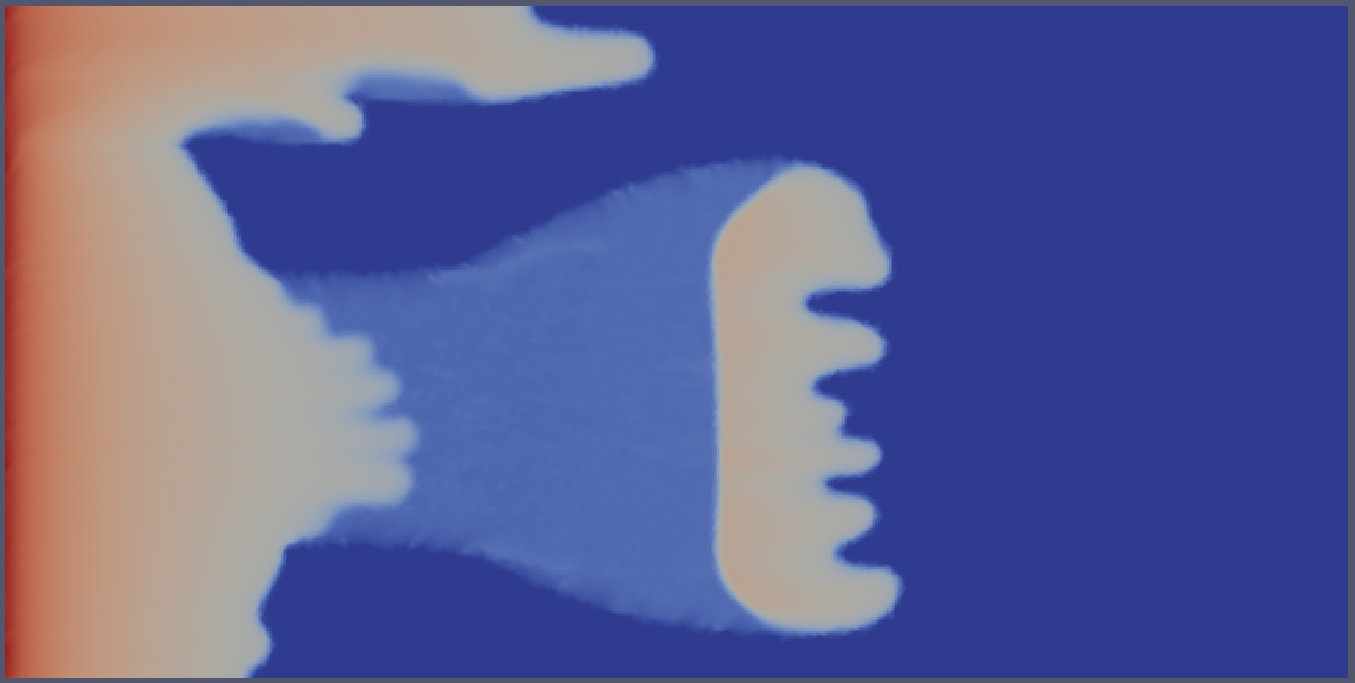
\includegraphics[width=.8\textwidth]{./Pics1/mr10_5regions_fixed/5regions_fixed_500.pdf} 
}
\vspace{0.0cm}
\hbox{\hspace{6.5cm} (a) flow at t=500 (fixed mesh)   
}
\vspace{0.25cm}
\hbox{\hspace{3.5cm}
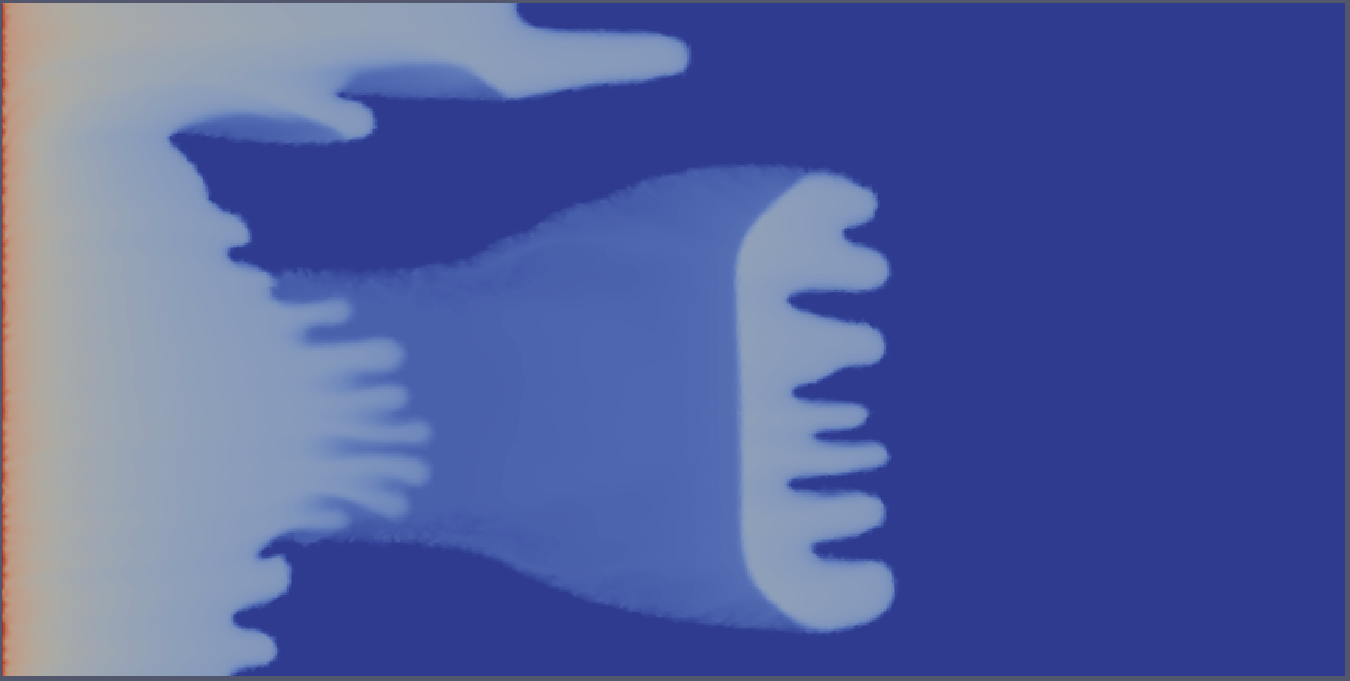
\includegraphics[width=.8\textwidth]{./Pics1/mr10_5regions_adapt/5regions_adapt_500.pdf}
}
\vspace{0.0cm}
\hbox{\hspace{6.5cm} (b) flow at t=500 (adaptive mesh)     
}
}     
\caption{At $time=0.25sec$ ($t=500$, timestemp) cross flow is taking place at the upper part of the formation. The fingers start to becoming more proufound for for the (b) case below.}
\label{fig:2testcase_b}
\end{figure}
\end{landscape}
\clearpage



%%%%
%%%%  FIGURE
%%%%
\begin{landscape}
\begin{figure}[ht] 
\vbox{
\hbox{\hspace{3.5cm}
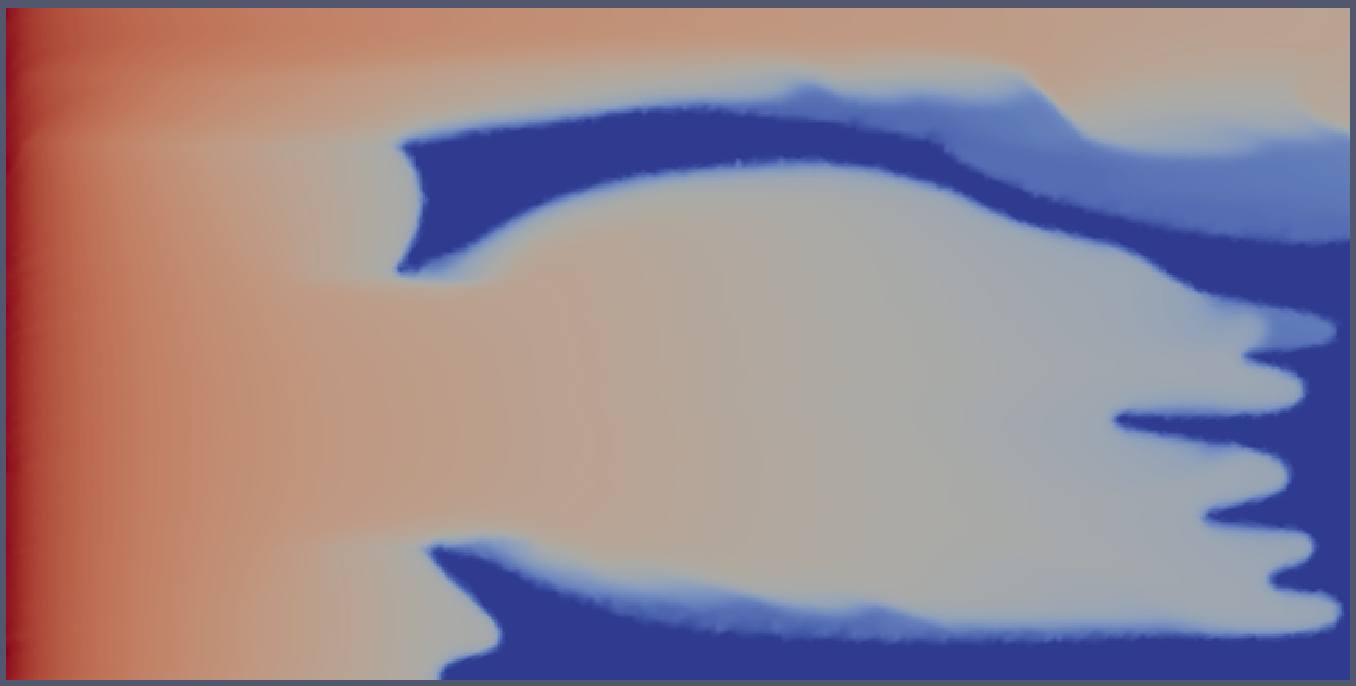
\includegraphics[width=.8\textwidth]{./Pics1/mr10_5regions_fixed/5regions_fixed_1500.pdf} 
}
\vspace{0.0cm}
\hbox{\hspace{6.5cm} (a) flow at t=1500 (fixed mesh)   
}
\vspace{0.25cm}
\hbox{\hspace{3.5cm}
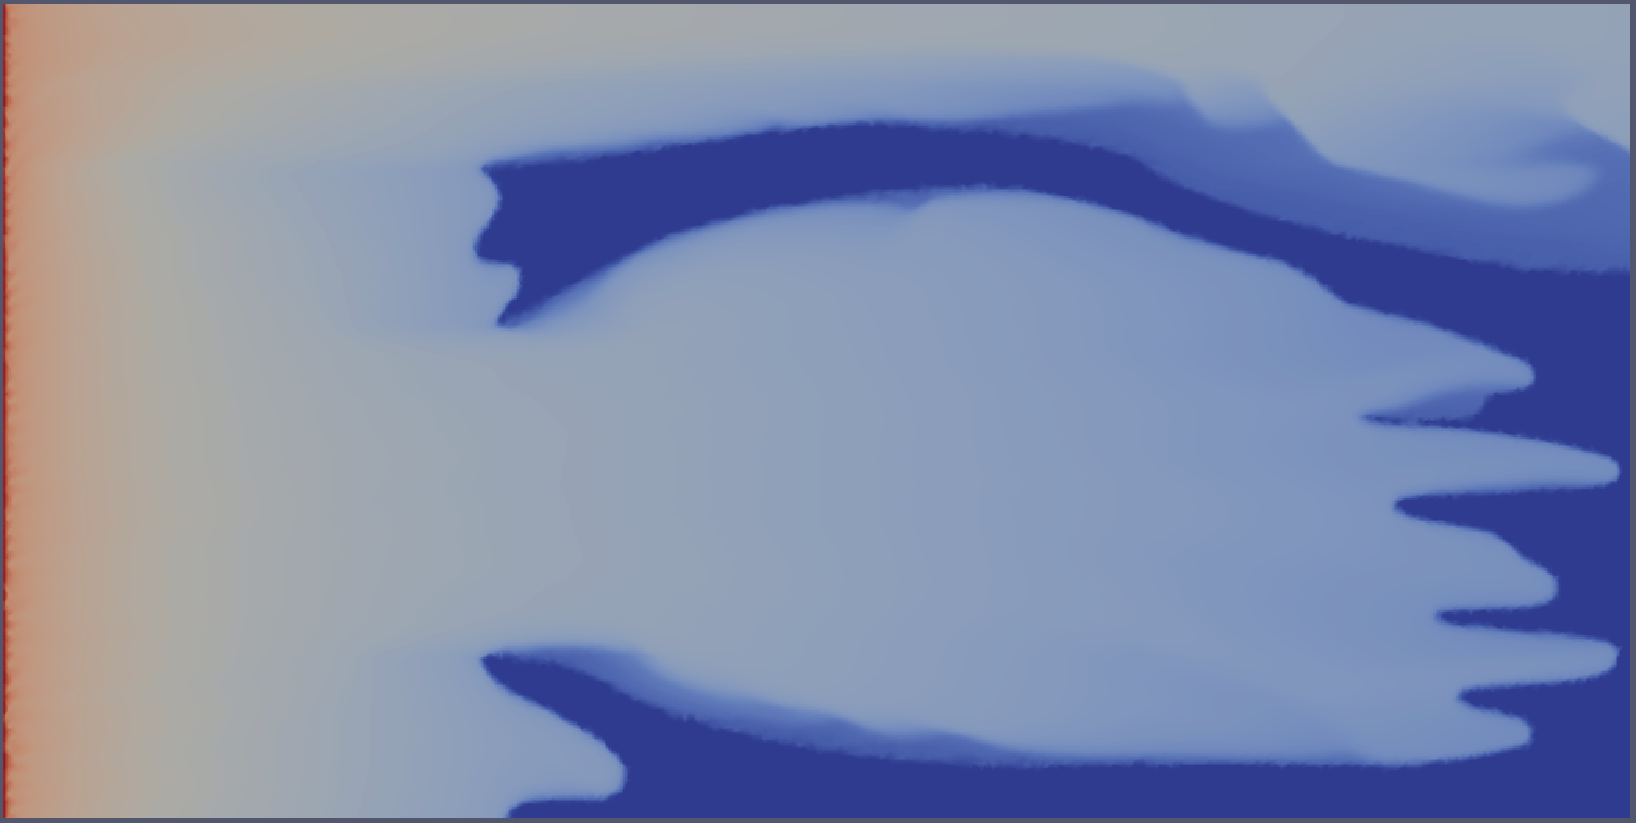
\includegraphics[width=.8\textwidth]{./Pics1/mr10_5regions_adapt/5regions_adapt_1500.pdf}
}
\vspace{0.0cm}
\hbox{\hspace{6.5cm} (b) flow at t=1500 (adaptive mesh)     
}
}     
\caption{At $time=0.75 sec$ ($t=1500$, timestemp) cross flow at the upper part has almost travel all the way towards the outlet (left-hand side) and the finger below start forming a front that is also travelling towards the left-hand side.}
\label{fig:2testcase_c}
\end{figure}
\end{landscape}
\clearpage



%%%%
%%%%  FIGURE
%%%%
\begin{landscape}
\begin{figure}[ht] 
\vbox{
\hbox{\hspace{3.5cm}
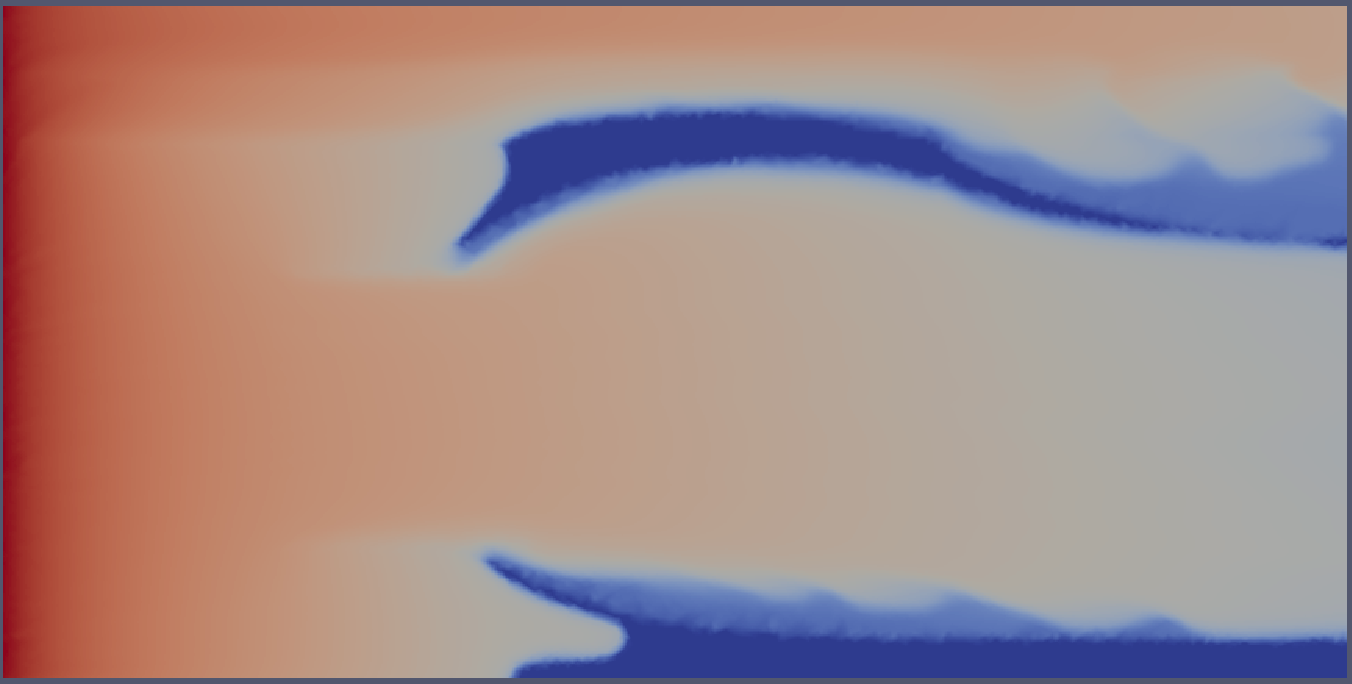
\includegraphics[width=.8\textwidth]{./Pics1/mr10_5regions_fixed/5regions_fixed_2000.pdf} 
}
\vspace{0.0cm}
\hbox{\hspace{6.5cm} (a) flow at t=end (fixed mesh)   
}
\vspace{0.25cm}
\hbox{\hspace{3.5cm}
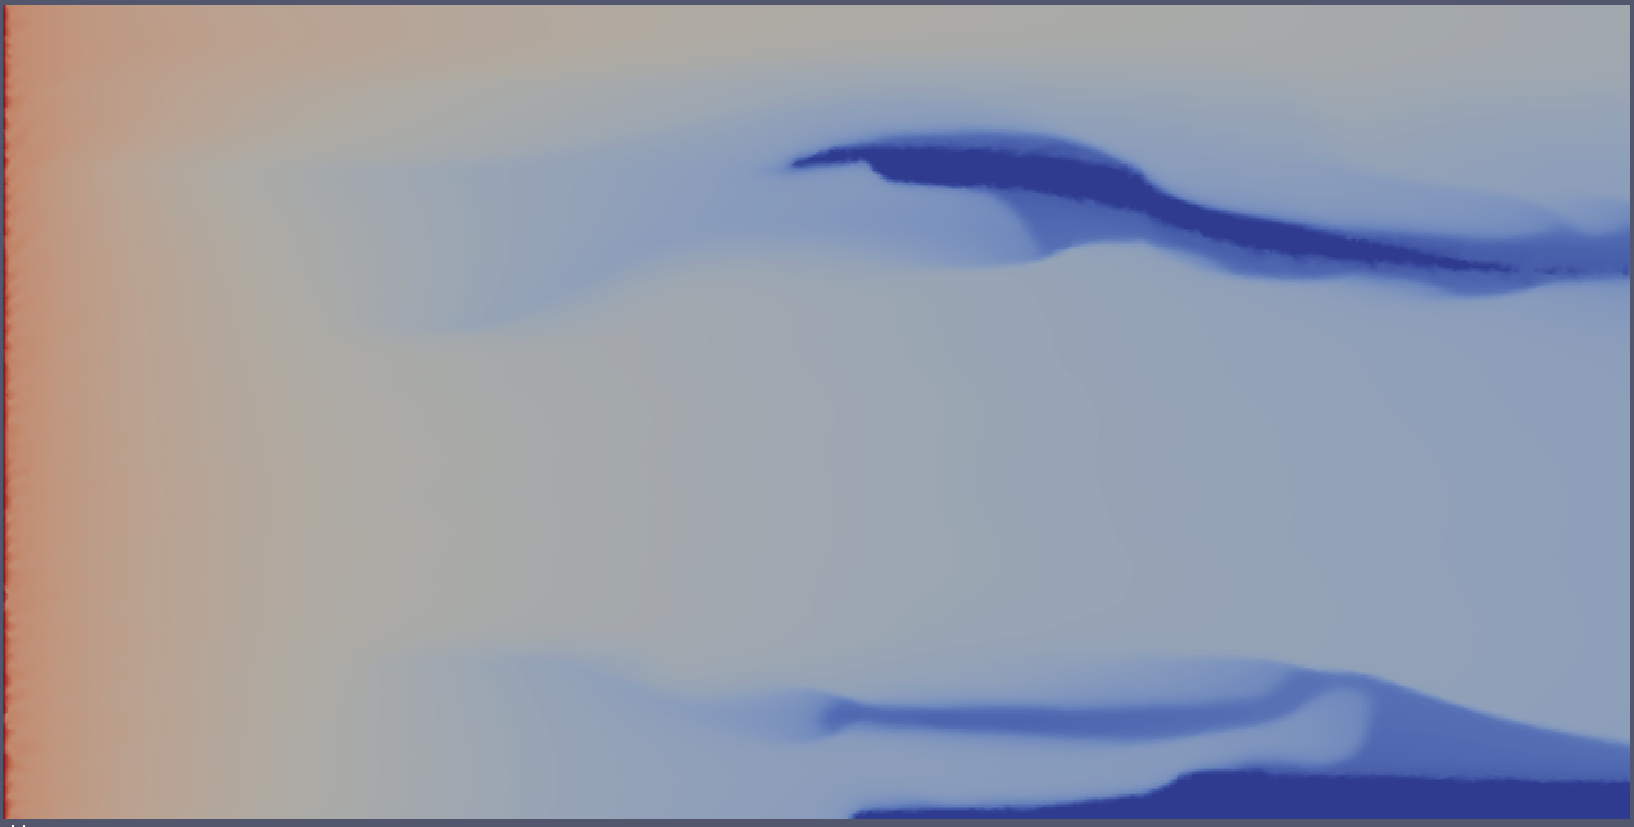
\includegraphics[width=.8\textwidth]{./Pics1/mr10_5regions_adapt/5regions_adapt_3000.pdf}
}
\vspace{0.0cm}
\hbox{\hspace{6.5cm} (b) flow at t=end (adaptive mesh)     
}
}     
\caption{Using the $P_{1}DGP_{2}$ element type for MR=$10$ under the same time steps, we compared the impact of fixed and adaptive mesh for the same timeframe. The end of simulation happens at $time=5 sec$ and for the timestemp $t=9999$ while the number of elements in both simulations was approximately $4700$. When adaptive mesh is introduce there is better repersentation of the fluid instabilities as these are developed on time.}
\label{fig:2testcase_d}
\end{figure}
\end{landscape}
\clearpage



%%%%
%%%%  FIGURE
%%%%
\begin{landscape}
\begin{figure}[ht] 
\vbox{
\hbox{\hspace{3.5cm}
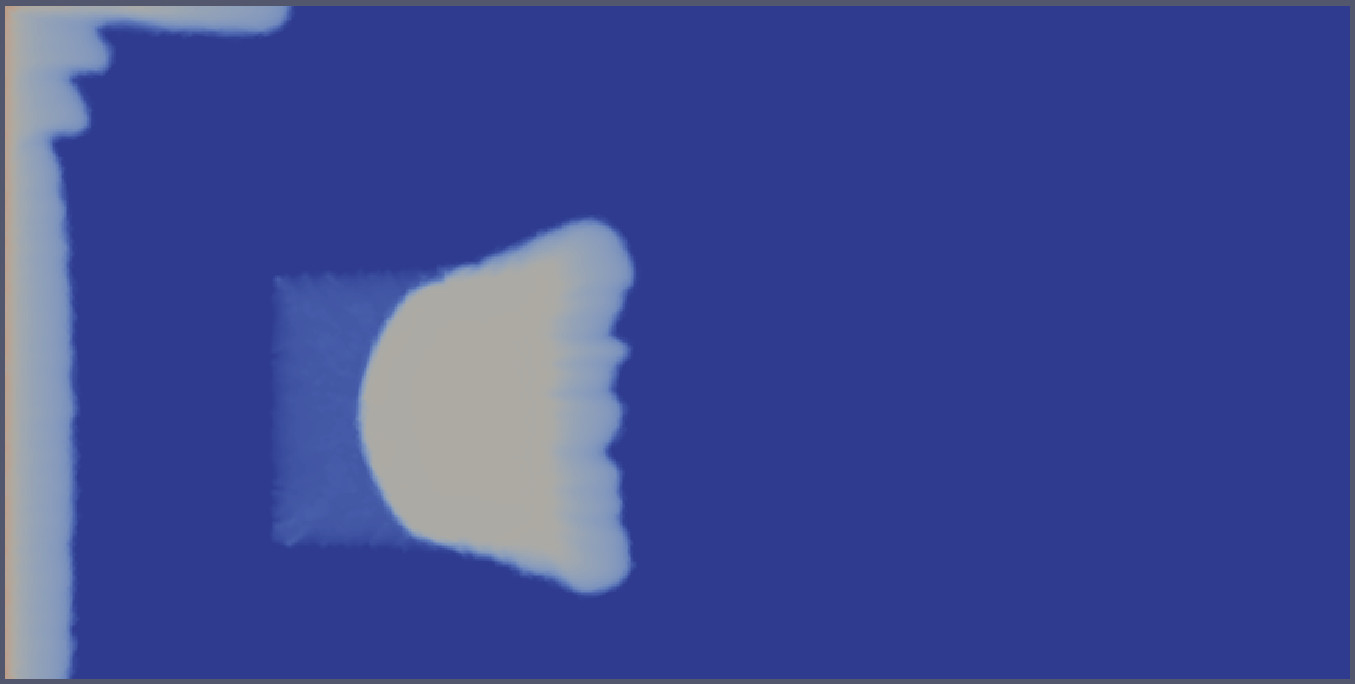
\includegraphics[width=.8\textwidth]{./Pics1/mr10_5regions_fixed_dinlet/5regions_dinlet_fixed_100}
}
\vspace{0.0cm}
\hbox{\hspace{6.5cm} (a) double inlet - fixed mesh   
}
\hbox{\hspace{3.5cm}
  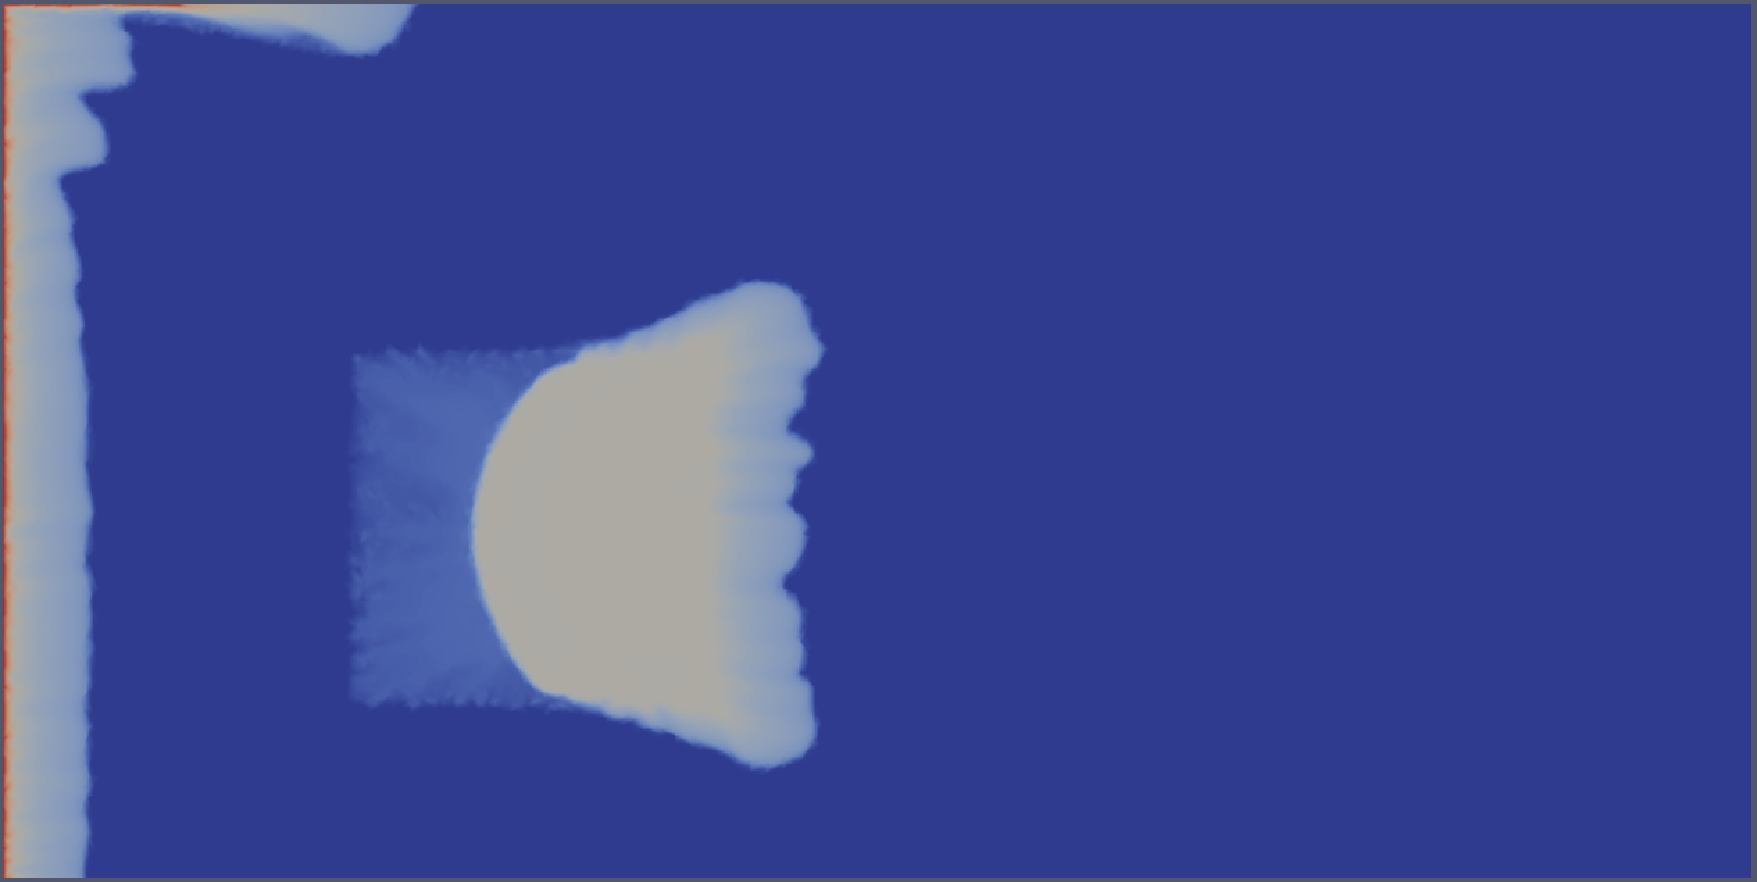
\includegraphics[width=.8\textwidth]{./Pics1/mr10_5regions_adapt_dinlet/5regions_dinlet_adapt_start}
}
\vspace{0.0cm}
\hbox{\hspace{6.5cm} (b) double inlet adaptive mesh   
}
}     
\caption{Comparing test-cases of fixed and adaptive mesh while we have a dual inlet, using the $P_{1}DGP_{2}$ element type for MR=$10$ under the same time steps}
\label{fig:3testcase_a}
\end{figure}
\end{landscape}
\clearpage

%%%%
%%%%  FIGURE
%%%%
\begin{figure}[ht] 
\vbox{
\hbox{\hspace{3.5cm}
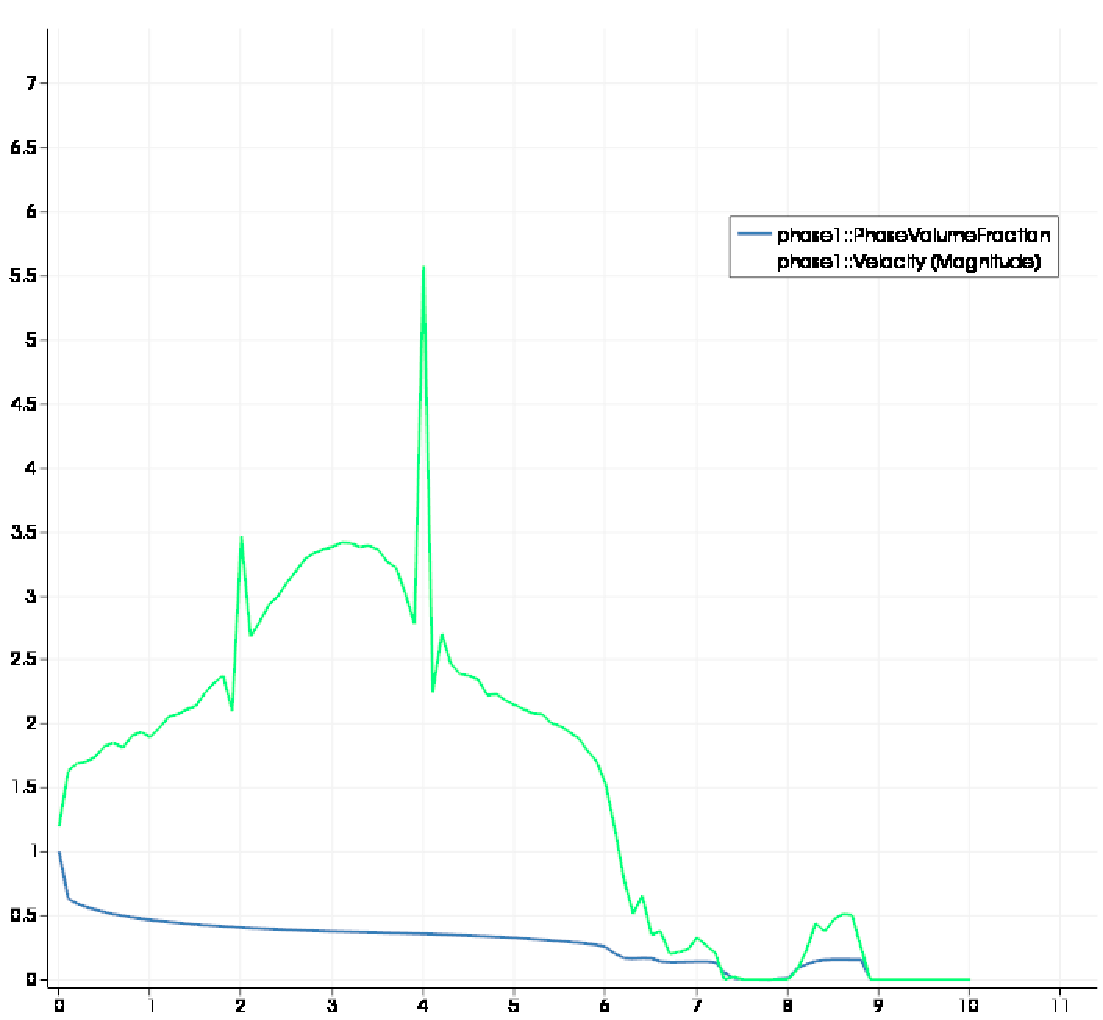
\includegraphics[width=.5\textwidth]{./Pics1/mr10_5regions_adapt/5regions_adapt_vel_magn.pdf} 
}
\vspace{0.0cm}
\hbox{\hspace{5.0cm} (a) single inlet velocity magnitude   
}
\hbox{\hspace{3.5cm}
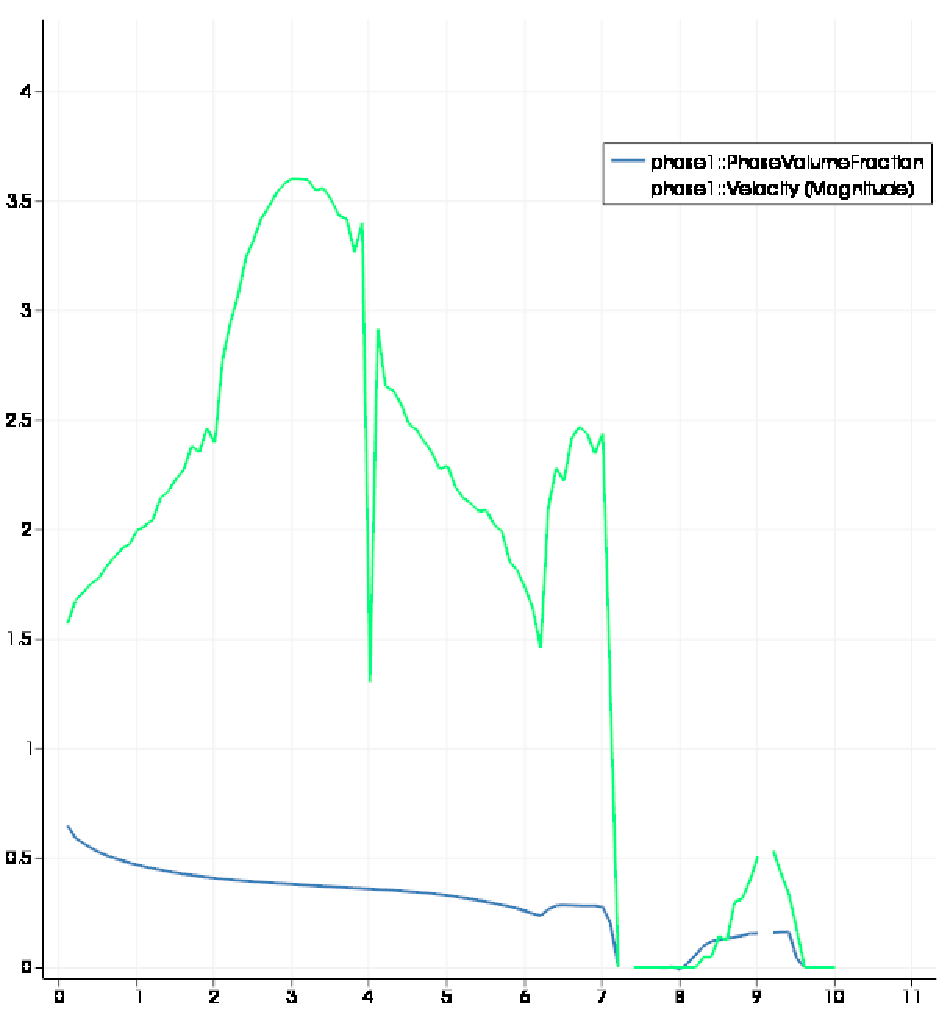
\includegraphics[width=.5\textwidth]{./Pics1/mr10_5regions_adapt_dinlet/5regions_dinlet_adapt_vel_magn.pdf}
}
\vspace{0.0cm}
\hbox{\hspace{5.0cm} (b) double inlet velocity magnitude   
}
}     
\caption{For the same time step, t=1000, these plots describe the velocity magnitudes of the phase $1$ (injected fluid) under the same boundary and initiall conditions. From top to bottom,these graphs describe the velocity magnitude %for fixed mesh is plotted(top), the velocity magnitude 
for adaptive mesh-single inlet (top) and the velocity magnitude for adaptive mesh with double inlet (bottom) as these are also presented in fig.\ref{fig:3testcase_a}. The main difference between the upper and lower plot %is not just the ability to capture in greater detail, the fluid instabilities as they happenduring the finger development and their velocity patterns. While there 
is the impact of the second injection interval as this can be seen from the slope and the rate that the velocity magnitude is changing.}
\label{fig:vel_magn}
\end{figure}

%%%%
%%%%  FIGURE
%%%%
\begin{landscape}
\begin{figure}[ht] 
\vbox{
\hbox{\hspace{3.5cm}
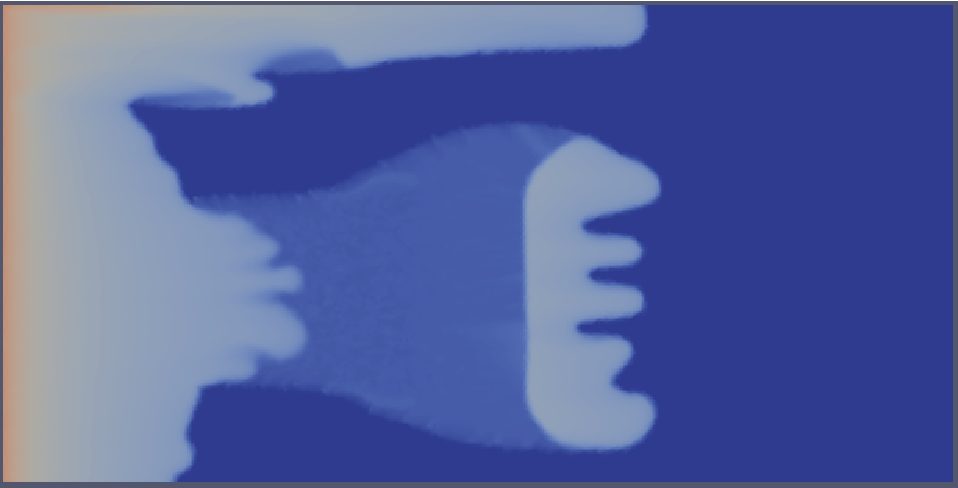
\includegraphics[width=.8\textwidth]{./Pics1/5reg_dinlet_fixed_500.pdf} 
}
\vspace{0.0cm}
\hbox{\hspace{6.5cm} (a) double inlet - fixed mesh   
}
\hbox{\hspace{3.5cm}
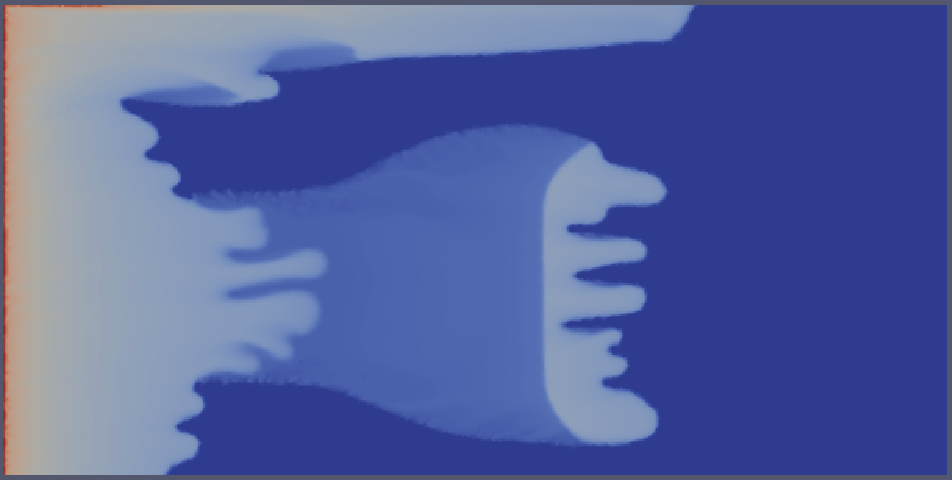
\includegraphics[width=.8\textwidth]{./Pics1/5reg_dinlet_adapt_500.pdf}
}
\vspace{0.0cm}
\hbox{\hspace{6.5cm} (b) double inlet adaptive mesh   
}
}     
\caption{for t=$500$ there is a comparison between fixed mesh(a) and adaptive mesh(b).}
\label{fig:3testcase_b}
\end{figure}
\end{landscape}
\clearpage

%%%%
%%%%  FIGURE
%%%%
\begin{landscape}
\begin{figure}[ht] 
\vbox{
\hbox{\hspace{3.5cm}
\includegraphics[width=.8\textwidth]{./Pics1/5reg_dinlet_fixed_1500.pdf} 
}
\vspace{0.0cm}
\hbox{\hspace{6.5cm} (a) double inlet - fixed mesh   
}
\hbox{\hspace{3.5cm}
\includegraphics[width=.8\textwidth]{./Pics1/5reg_dinlet_adapt_1500.pdf}
}
\vspace{0.0cm}
\hbox{\hspace{6.5cm} (b) double inlet adaptive mesh   
}
}     
\caption{for t=$1500$ there is a comparison between fixed mesh(a) and adaptive mesh(b).}
\label{fig:3testcase_c}
\end{figure}
\end{landscape}
\clearpage

%%%%
%%%%  FIGURE
%%%%
\begin{landscape}
\begin{figure}[ht] 
\vbox{
\hbox{\hspace{3.5cm}
\includegraphics[width=.8\textwidth]{./Pics1/5reg_dinlet_fixed_end.pdf} 
}
\vspace{0.0cm}
\hbox{\hspace{6.5cm} (a) double inlet - fixed mesh   
}
\hbox{\hspace{3.5cm}
\includegraphics[width=.8\textwidth]{./Pics1/5reg_dinlet_adapt_end.pdf}
}
\vspace{0.0cm}
\hbox{\hspace{6.5cm} (b) double inlet adaptive mesh   
}
}     
\caption{for t=$1500$ there is a comparison between fixed mesh(a) and adaptive mesh(b).}
\label{fig:3testcase_d}
\end{figure}
\end{landscape}
\clearpage

%%%%
%%%%  FIGURE
%%%%
\begin{landscape}
\begin{figure}[ht] 
\vbox{
\hbox{\hspace{3.5cm}
\includegraphics[width=.8\textwidth]{./Pics1/mr100_fixed/mr100_fixed_500.pdf} 
}
\vspace{0.0cm}
\hbox{\hspace{4.0cm} (a) fixed and unstructured mesh for MR = 100 (start)   
}
\hbox{\hspace{3.5cm}
\includegraphics[width=.8\textwidth]{./Pics1/mr100_fixed/mr100_fixed_1500.pdf}
}
\vspace{0.0cm}
\hbox{\hspace{3.75cm} (b) fixed and unstructured mesh for MR = 100 (t = 1500)   
}
}     
\caption{For the case of MR=$100$ from top to bottom, the number of elements is $4680$ and fixed and unstructured mesh for the same time steps, t=$0.25$ or t=500(a), t=$0.75$ or t=1500(b). }
\label{fig:4testcase_a}
\end{figure}
\end{landscape}
\clearpage

%%%%
%%%%  FIGURE
%%%%
\begin{landscape}
\begin{figure}[ht] 
\vbox{
\hbox{\hspace{3.5cm}
\includegraphics[width=.8\textwidth]{./Pics1/mr100_fixed/mr100_fixed_3000.pdf} 
}
\vspace{0.0cm}
\hbox{\hspace{3.75cm} (c) fixed and unstructured mesh for MR = 100    
}
\hbox{\hspace{3.5cm}
\includegraphics[width=.8\textwidth]{./Pics1/mr100_fixed/mr100_fixed_end.pdf}
}
\vspace{0.0cm}
\hbox{\hspace{7.cm} (d) end of simulations     
}
}     
\caption{screenshot (c) is for t=$1.5$ sec or t=$3000$ and screenshot (d) is for t=$3.175$ sec, at the end of the simulations. }
\label{fig:4testcase_b}
\end{figure}
\end{landscape}
\clearpage

